%% Version 4.3.2, 25 August 2014
%
%%%%%%%%%%%%%%%%%%%%%%%%%%%%%%%%%%%%%%%%%%%%%%%%%%%%%%%%%%%%%%%%%%%%%%
% Template.tex --  LaTeX-based template for submissions to the 
% American Meteorological Society
%
% Template developed by Amy Hendrickson, 2013, TeXnology Inc., 
% amyh@texnology.com, http://www.texnology.com
% following earlier work by Brian Papa, American Meteorological Society
%
% Email questions to latex@ametsoc.org.
%
%%%%%%%%%%%%%%%%%%%%%%%%%%%%%%%%%%%%%%%%%%%%%%%%%%%%%%%%%%%%%%%%%%%%%
% PREAMBLE
%%%%%%%%%%%%%%%%%%%%%%%%%%%%%%%%%%%%%%%%%%%%%%%%%%%%%%%%%%%%%%%%%%%%%

%% Start with one of the following:
% DOUBLE-SPACED VERSION FOR SUBMISSION TO THE AMS
\documentclass{ametsoc}

% TWO-COLUMN JOURNAL PAGE LAYOUT---FOR AUTHOR USE ONLY
% \documentclass[twocol]{ametsoc}

%%%%%%%%%%%%%%%%%%%%%%%%%%%%%%%%
%%% To be entered only if twocol option is used

\journal{jas}

%  Please choose a journal abbreviation to use above from the following list:
% 
%   jamc     (Journal of Applied Meteorology and Climatology)
%   jtech     (Journal of Atmospheric and Oceanic Technology)
%   jhm      (Journal of Hydrometeorology)
%   jpo     (Journal of Physical Oceanography)
%   jas      (Journal of Atmospheric Sciences)	
%   jcli      (Journal of Climate)
%   mwr      (Monthly Weather Review)
%   wcas      (Weather, Climate, and Society)
%   waf       (Weather and Forecasting)
%   bams (Bulletin of the American Meteorological Society)
%   ei    (Earth Interactions)

%%%%%%%%%%%%%%%%%%%%%%%%%%%%%%%%
%Citations should be of the form ``author year''  not ``author, year''
\bibpunct{(}{)}{;}{a}{}{,}

%%%%%%%%%%%%%%%%%%%%%%%%%%%%%%%%

%%% To be entered by author:

%% May use \\ to break lines in title:

\title{Tropopause Evolution in a Rapidly Intensifying Tropical Cyclone: A Static Stability Budget Analysis in an Idealized, Axisymmetric Framework}

%%% Enter authors' names, as you see in this example:
%%% Use \correspondingauthor{} and \thanks{Current Affiliation:...}
%%% immediately following the appropriate author.
%%%
%%% Note that the \correspondingauthor{} command is NECESSARY.
%%% The \thanks{} commands are OPTIONAL.

    %\authors{Author One\correspondingauthor{Author One, 
    % American Meteorological Society, 
    % 45 Beacon St., Boston, MA 02108.}
% and Author Two\thanks{Current affiliation: American Meteorological Society, 
    % 45 Beacon St., Boston, MA 02108.}}

\authors{Patrick Duran\correspondingauthor{Department of Atmospheric and Environmental Sciences, University at Albany, State University of New York, 1400 Washington Avenue, Albany, NY.} and John Molinari}

%% Follow this form:
    % \affiliation{American Meteorological Society, 
    % Boston, Massachusetts.}

\affiliation{University at Albany, State University of New York,
Albany, NY}

%% Follow this form:
    %\email{latex@ametsoc.org}

\email{pduran2008@gmail.com}

%% If appropriate, add additional authors, different affiliations:
    %\extraauthor{Extra Author}
    %\extraaffil{Affiliation, City, State/Province, Country}

%\extraauthor{}
%\extraaffil{}

%% May repeat for a additional authors/affiliations:

%\extraauthor{}
%\extraaffil{}

%%%%%%%%%%%%%%%%%%%%%%%%%%%%%%%%%%%%%%%%%%%%%%%%%%%%%%%%%%%%%%%%%%%%%
% ABSTRACT
%
% Enter your abstract here
% Abstracts should not exceed 250 words in length!
%
% For BAMS authors only: If your article requires a Capsule Summary, please place the capsule text at the end of your abstract
% and identify it as the capsule. Example: This is the end of the abstract. (Capsule Summary) This is the capsule summary. 

\abstract{Large changes in tropopause-layer static stability are observed during the rapid intensification (RI) of an idealized, axisymmetric tropical cyclone (TC).
Over the eye, static stability near the tropopause decreases and the cold-point tropopause height rises by up to 4 km at the storm center.
Outside of the eye, static stability increases considerably just above the cold-point tropopause, and the tropopause remains near its initial level.\\
\indent A budget analysis reveals that the advection term, which includes differential advection of potential temperature and direct advection of static stability, is important throughout the upper troposphere and lower stratosphere.
Within the eye, differential advection plays a particularly important role in destabilizing the layer near and above the cold-point tropopause.
Outside of the eye, a radial-vertical circulation develops during RI, with strong outflow below the tropopause and weak inflow above.
The upper-tropospheric outflow layer exports high potential temperature ($\theta$) air from the eyewall to large radii in the upper troposphere.
This increase in $\theta$ forces stabilization below the outfow jet and destabilization above.
Vertical wind shear above and below the upper-tropospheric outflow maximum induces vertical gradients of turbulence, which also modify the vertical stability profile.
Meanwhile, as organized convection reaches the tropopause, radiative heating tendencies at the top of the cirrus canopy generally act to destabilize the upper troposphere and stabilize the lower stratosphere.
Turbulent mixing and radiative heating combine to play an important role in the development of the strong stable layer immediately above the cold-point tropopause during RI.}
%The results suggest that turbulence and radiation, alongside advection, play fundamental roles in the upper-level static stability evolution of TCs.}
%The conclusions are robust to changes in the initial thermodynamic profile and prescribed vertical mixing length within a reasonable range of values.}

\begin{document}

%% Necessary!
\maketitle


%%%%%%%%%%%%%%%%%%%%%%%%%%%%%%%%%%%%%%%%%%%%%%%%%%%%%%%%%%%%%%%%%%%%%
% MAIN BODY OF PAPER
%%%%%%%%%%%%%%%%%%%%%%%%%%%%%%%%%%%%%%%%%%%%%%%%%%%%%%%%%%%%%%%%%%%%%
%

%% In all cases, if there is only one entry of this type within
%% the higher level heading, use the star form: 
%%
 \section{Introduction}

%Perhaps introduce upper-tropospheric static stability and its relationship to the diurnal cycle before going into Patricia? Include references to Dunion, Navarro, and O'Neill here.
%More recently, \cite{Dunionetal2014} documented a periodic oscillation of infrared brightness temperature in hurricanes, which they call the "TC diurnal pulse."
%There will be a whole bunch of papers cited here...
%At some point (probably in the Discussion) mention the possible importance of static stability asymmetries, in the context of the Dunion diurnal pulse 

Using a high-resolution dropsonde dataset collected during the Tropical Cyclone Intensity experiment (TCI; \citeauthor{DoyleTCI} \citeyear{DoyleTCI}), \cite{DuranMolinari2018} observed dramatic changes in tropopause structure during the rapid intensification (RI) of Hurricane Patricia (2015).
The goal of the present paper is to analyze the processes that might have produced the upper-tropospheric and lower-stratospheric fluctuations observed in Patricia using an idealized axisymmetric simulation.

After undergoing a remarkably rapid intensification (RI), Hurricane Patricia (2015) set a new record as the strongest tropical cyclone (TC) ever observed in the Western Hemisphere (\citeauthor{Kimberlainetal2016} \citeyear{Kimberlainetal2016}; \citeauthor{Rogersetal2017} \citeyear{Rogersetal2017}).
%High-altitude dropsonde observations taken during the Tropical Cyclone Intensity (TCI) experiment captured this RI in unprecedented detail \citep{DoyleTCI}.
TCI dropsonde observations collected during this RI period revealed dramatic changes in the cold-point tropopause height and upper-level static stability \citep{DuranMolinari2018}.
In particular, when Patricia was at tropical storm intensity shortly before RI commenced, a strong inversion layer existed just above the cold-point tropopause.
During the first half of the RI period, this inversion layer weakened throughout Patricia's inner core, with the weakening most pronounced over the developing eye.
By the time the storm reached its maximum intensity of 95 m s\textsuperscript{-1}, the inversion layer over the eye had disappeared almost completely, which was accompanied by a greater than 1-km increase in the tropopause height.
Meanwhile over the eyewall region, the static stability increased and the tropopause remained near its initial level.
%The mechanisms that might have led to this tropopause-layer variability will be investigated in the current paper using idealized simulations.

Despite the importance of tropopause-layer thermodynamics in theoretical models of hurricanes (\citeauthor{EmanuelRotunno2011} \citeyear{EmanuelRotunno2011}; \citeauthor{Emanuel2012} \citeyear{Emanuel2012}), most observational studies of the upper-tropospheric structure of TCs are decades old.
Recently, however, \cite{KomaromiDoyle2017} found that stronger TCs tended to have a higher and warmer tropopause over their inner core than weaker TCs.
Their results are consistent with the evolution observed over the inner core of Hurricane Patricia, in which the tropopause height increased and the tropopause temperature warmed throughout RI \citep{DuranMolinari2018}.

An idealized simulations of a TC analyzed by \cite{OhnoSatoh2015} suggested that the development of an upper-level warm core near the 13-km level acted to decrease the static stability near the tropopause within the eye.
During the early stage of development in their simulation (their Fig. 9), static stability above 16 km was large at all radii.
However, after the storm's intensification, the static stability above 16 km within the eye was markedly smaller (their Fig. 10c).
Although the mechanisms that might drive this static stability evolution have not been examined explicitly it might be related to the development of an upper-tropospheric warm care within the eye.
\cite{SternZhang2013} described the development of the TC warm core using a potential temperature ($\theta$) budget analysis.
Although the warm anomaly in their simulation maximized in the mid-levels, they also note that a secondary warming maximum existed in the 12-14-km layer.
They found that radial and vertical advection both played important roles in warm core development throughout RI, and subgrid-scale diffusion became particularly important during the later stage of RI.
The warming of the upper troposophere by these advective and diffusive processes could contribute to a decrease in static stability near the tropoopause within the eye.
Other processes that can modify the static stability in the upper troposphere of TCs include radiative heating within and near the top of the cirrus canopy and shear-induced turbulent mixing near the outflow jet.

To our knowledge, the only paper that has examined explicitly the static stability evolution in a modeled TC is \cite{Kepertetal2016}, but their analysis was limited to the boundary layer.
The analysis herein is based upon that of \cite{SternZhang2013}, except using a static stability budget similar to that of \cite{Kepertetal2016}, with a focus on the upper-tropospheric and lower-stratospheric evolution during RI.

 \section{Model Setup}

The numerical simulations were performed using version 19.4 of Cloud Model 1 (CM1) described in \cite{BryanRotunno2009}.
The equations of motion were integrated on a 3000-km-wide, 30-km-deep axisymmetric grid with 1-km horizontal and 250-m vertical grid spacing.
The computations were performed on an \textit{f}-plane at 15\textdegree{N} latitude, over a sea surface with constant temperature of 30.5\textdegree C, which matches that observed near Hurricane Patricia (2015; \citeauthor{Kimberlainetal2016} \citeyear{Kimberlainetal2016}).
Horizontal turbulence was parameterized using the Smagorinsky scheme described in \citeauthor{BryanRotunno2009} (\citeyear{BryanRotunno2009}, pg. 1773), with a prescribed mixing length that varied linearly from 100 m at a surface pressure of 1015 hPa to 1000 m at a surface pressure of 900 hPa.
Vertical turbulence was parameterized using the formulation of \citeauthor{MarkowskiBryan2016} (\citeyear{MarkowskiBryan2016}, their Eq. 6), using an asymptotic vertical mixing length of 100 m.
A Rayleigh damping layer was applied outside of the 2900-km radius and above the 25-km level to prevent spurious gravity wave reflection at the model boundaries.
Microphysical processes were parameterized using the \cite{Thompson} scheme and radiative heating tendencies were computed every two minutes using the Rapid Radiative Transfer Model for GCMs (RRTMG) longwave and shortwave schemes \citep{Iacono}.
The initial temperature and humidity field was horizontally homogeneous and determined by averaging all Climate Forecast System Reanalysis (CFSR) grid points within 100 km of Patricia's center of circulation at 18 UTC 21 October 2015.
%A horizontally-homogeneous temperature and humidity field was initialized with a mean sounding computed using all dropsondes deployed during the TCI flight conducted within and around Tropical Storm Patricia on 21 October, 2015 (see \citeauthor{DoyleTCI} \citeyear{DoyleTCI} for details.)
%Above 19 km, where few TCI observations were available, the temperature profile was taken from the Climate Forecast System Reanalysis (CFSR) grid point nearest Patricia's storm center, valid at 18 UTC 21 October, 2015.
%Since relative humidity measurements were unreliable at temperatures below -40\textdegree C \citep{BellTCI}, relative humidity was set equal to 50\% above 11.5 km (the level above which temperature dropped below -40\textdegree C).
The vortex described in \citeauthor{RotunnoEmanuel} (\citeyear{RotunnoEmanuel}, their Eq. 37) was used to initialize the wind field, setting all parameters equal to the values used therein.

Although hurricanes simulated in an axisymmetric framework tend to be more intense than those observed in nature, the intensity evolution of this simulation matches reasonably well with that observed in Hurricane Patricia.
After an initial spin-up period of about 20 hours, the modeled storm (Fig.~\ref{fig:vmax+pmin}, blue lines) began an RI period that lasted approximately 30 hours.
After this RI, the storm continued to intensify more slowly until the maximum 10-m wind speed reached 89 m s\textsuperscript{-1} and the sea-level pressure reached its minimum of 846 hPa 81 hours into the simulation.
Hurricane Patricia (red stars) exhibited a similar intensity evolution prior to its landfall, with an RI period leading to a maximum 10-m wind speed of 95 m s\textsuperscript{-1} and a minimum sea-level pressure of 872 hPa.

 \section{Budget Computation}

The static stability can be expressed as the squared Brunt-V{\"a}is{\"a}l{\"a} frequency:
   \begin{equation} \label{eq:n2moist}
   N_m^2 = \frac{g}{T}\left(\frac{\partial T}{\partial z}+\Gamma_m\right)\left(1+\frac{T}{R_d/R_v+q_s}\frac{\partial q_s}{\partial T}\right)-\frac{g}{1+q_t}\frac{\partial q_t}{\partial z},
   \end{equation}
where $g$ is gravitational acceleration, $T$ is temperature, $R_d$ and $R_v$ are the gas constants of dry air and water vapor, respectively, $q_s$ is the saturation mixing ratio, $q_t$ is the total condensate mixing ratio, and $\Gamma_m$ is the moist-adiabatic lapse rate:
   \begin{equation} \label{eq:gamma_m}
   \Gamma_m = g(1+q_t)\left(\frac{1+L_vq_s/R_dT}{c_p_m +L_v\partial q_s/\partial T}\right),
   \end {equation}
where $L_v$ is the latent heat of vaporization and $c_{pm}$ is the specific heat of moist air at constant pressure.
In the tropopause layer, $q_s$, ${\partial q_s}/{\partial T}$, and ${\partial q_t}/{\partial z}$ approach zero. In this limiting case, Eq. \ref{eq:n2moist} reduces to:
   \begin{equation} \label{eq:n2dry}
   N^2 = \frac{g}{\theta}\frac{\partial \theta}{\partial z},
   \end{equation}
where $\theta$ is the potential temperature.

To compute $N^2$, CM1 uses Eq. \ref{eq:n2moist} in saturated environments and Eq. \ref{eq:n2dry} in sub-saturated environments. For simplicity, however, only Eq. \ref{eq:n2dry} will be employed for the budget computations throughout the entire domain\footnote{The validity of this approximation will be substantiated later in this section.}.

Taking the time derivative of Eq. \ref{eq:n2dry} yields the static stability tendency:
   \begin{equation} \label{eq:dn2dt}
   \frac{\partial N^2}{\partial t} = \frac{g}{\theta}\frac{\partial}{\partial z}\frac{\partial \theta}{\partial t}-\frac{g}{\theta^2}\frac{\partial \theta}{\partial z}\frac{\partial \theta}{\partial t},
   \end{equation}
where the potential temperature tendency, $\partial \theta/\partial t$, can be written, following \cite{Bryan2017}:
   \begin{equation} \label{eq:dthetadt}
%   \frac{\partial \theta}{\partial t} = HADV+VADV+HTURB+VTURB+MP+RAD+DISS 
   \frac{\partial \theta}{\partial t} = -u\frac{\partial\theta}{\partial r}-w\frac{\partial \theta}{\partial z}+HTURB+VTURB+MP+RAD+DISS
   \end{equation}
Each term on the right-hand side of Eq.~\ref{eq:dthetadt} represents a $\theta$ budget variable, each of which is output directly by the model every minute.

The first term on the right-hand side of Eq. ~\ref{eq:dn2dt} is larger than the second term throughout most of the tropopause layer (not shown).
Consequently, the contribution of each of the terms in Eq.~\ref{eq:dthetadt} to the $N^2$ tendency can be interpreted in light of a vertical gradient of each term.
%Since the first term on the right-hand side of Eq.~\ref{eq:dn2dt} is larger than the second term throughout most of the tropopause layer (not shown), the contribution of each of the terms in Eq.~\ref{eq:dthetadt} to the $N^2$ tendency can be interpreted in light of a vertical gradient of each term.

Taking the vertical gradient of the first two terms on the right-hand side of Eq.~\ref{eq:dthetadt} yields the time tendency of the vertical $\theta$ gradient due to horizontal and vertical advection\footnote{These terms include the tendencies due to implicit diffusion in the fifth-order finite differencing scheme, which are separated from the advection terms in the CM1 budget output}:

   \begin{equation} \label{eq:advtend}
   \left(\frac{\partial}{\partial t}\frac{\partial \theta}{\partial z}\right)_{adv} = -u\frac{\partial}{\partial r}\frac{\partial \theta}{\partial z}-w\frac{\partial}{\partial z}\frac{\partial \theta}{\partial z}-\frac{\partial u}{\partial z}\frac{\partial \theta}{\partial r}-\frac{\partial w}{\partial z}\frac{\partial \theta}{\partial z}.
   \end{equation}
The first two terms on the right-hand side of Eq.~\ref{eq:advtend} represent advection of static stability by the radial and vertical wind, respectively.
These terms act to rearrange the static stability field, but cannot strengthen or weaken static stability maxima or minima.
The third and fourth terms on the right-hand side of Eq.~\ref{eq:advtend} represent, respectively, the tilting of isentropes in the presence of vertical wind shear, and the stretching or squashing of isentropes by vertical gradients of vertical velocity.
Since these terms involve velocity gradients, they can act to strengthen or weaken static stability maxima or minima through differential advection.
Unless otherwise stated, any reference to "advection" in this paper indicates the sum of all of the terms in Eq.~\ref{eq:advtend}.
%For example, since the $\theta$ of the air flowing out of the eyewall into the upper-tropospheric outflow layer increases as the TC intensifies, $\theta$ increases locally within the outflow layer.
%This acts to increase $\partial \theta/\partial z$ below the outflow maximum and decrease $\partial \theta/\partial z$ above, thereby modifying the static stability field.
%Similarly, the decay of updrafts with height at the top of convective towers can act to increase $\partial \theta/\partial z$ through squashing of isentropes.

Returning to Eq.~\ref{eq:dthetadt}, HTURB and VTURB are the $\theta$ tendencies from the horizontal and vertical turbulence parameterizations, MP is the tendency from the microphysics scheme, RAD is the tendency from the radiation scheme, and DISS is the tendency due to turbulent dissipation.
This equation neglects Rayleigh damping, since the entire analysis domain lies outside of the regions where damping is applied.
Each term in Eq. \ref{eq:dthetadt} is substituted for ${\partial \theta}/{\partial t}$ in Eq. \ref{eq:dn2dt}, yielding the contribution of each budget term to the static stability tendency.
These terms are summed, yielding an instantaneous "budget change" in $N^2$ every minute.
The budget changes are then averaged over 24-hour periods and compared to the total model change in $N^2$ over that same time period, i.e.:
   \begin{equation} \label{eq:budgetchange}
   \Delta N^2_{budget} = \frac{1}{\delta t}\sum_{t=t_0}^{t_0+\delta t} \left.\frac{\partial N^2}{\partial t}\right\vert_t
   \end{equation}
   \begin{equation} \label{eq:modelchange}
   \Delta N^2_{model} = N^2_{t_0+\delta t}-N^2_{t_0}
   \end{equation}
   \begin{equation} \label{eq:residual}
   Residual = \Delta N^2_{model}-\Delta N^2_{budget}
   \end{equation}
where $t_0$ is an initial time and $\delta t$ is 24 hours.

Eqs. \ref{eq:budgetchange}-\ref{eq:residual} are plotted for three consecutive 24-hour periods in Fig.~\ref{fig:mod+bud+res}.
For this and all subsequent radial-vertical cross sections, a 1-2-1 smoother is applied once in the radial direction to eliminate $2\Delta r$ noise that appears in some of the raw model output and calculated fields.
      The left column of Fig.~\ref{fig:mod+bud+res} depicts the model changes computed using Eq.~\ref{eq:modelchange}, together with Eq.~\ref{eq:n2moist} in saturated environments and Eq. \ref{eq:n2dry} in subsaturated environments.
The center column depicts the budget changes computed using Eq. \ref{eq:budgetchange} together with Eq.~\ref{eq:n2dry} throughout the entire domain.
Thus, the left column includes the effect of moisture in the $N^2$ computations, whereas the center column neglects moisture.
The right column depicts the residuals, computed using Eq. \ref{eq:residual} (i.e. the left column minus the center column.)
In every 24-hour period, the budget changes are nearly identical to the model changes, which is reflected in the near-zero residuals in the right column.
This indicates that the budget accurately represents the model variability, which implies that the neglect of moisture in the budget computation introduces negligible error within the analysis domain\footnote{This is not the case in the lower- and mid-troposphere, where the residual actually exceeds the budget tendencies in many places, likely due to the neglect of moisture; thus we limit this analysis to the upper troposphere and lower stratosphere.}.

In the tropopause layer, some of the budget terms are small enough to be ignored.
To determine which of the budget terms are most important, a time series of the contribution of each of the budget terms in Eq. \ref{eq:dthetadt} to the tropopause-layer static stability tendency is plotted in Fig.~\ref{fig:avgbudterms}.
For this figure, each of the budget terms is computed using the method described in Section 3, except with 1-hour averaging intervals instead of 24-hour intervals.
The absolute values of these tendencies are then averaged over the radius-height domain of the plots shown in Fig.~\ref{fig:mod+bud+res} and plotted as a time series\footnote{It will be seeen in subsequent figures that each of the terms contributes both positively and negatively to the $N^2$ tendency within the analysis domain. 
Thus, taking an average over the domain tends to wash out the positive and negative contributions.
To circumvent this problem, the absolute value of each of the terms is averaged.}. 
Advection (Fig.~\ref{fig:avgbudterms}, red line) plays an important role in the mean tropopause-layer static stability tendency at all times, and vertical turbulence (Fig.~\ref{fig:avgbudterms}, blue line) and radiation (Fig.~\ref{fig:avgbudterms}, dark green line) also contribute significantly.
The remaining three processes - horizontal turbulence, microphysics, and dissipative heating -  are negligible everywhere outside of the eyewall, and do not play important roles in the mesoscale tropopause variability.

The preceding analysis indicates that, at all times, three budget terms dominate the tropopause-layer static stability tendency: advection, vertical turbulence, and radiation.
Variations in the magnitude and spatial structure of these terms drive the static stability changes depicted in Fig.~\ref{fig:mod+bud+res}; subsequent sections will focus on these variations and what causes them.

 \section{Results}

 \subsection{Static stability evolution}

The average $N^2$ over the first day of the simulation (Fig.~\ref{fig:n2-24hr-avgs}a) indicates the presence of a weak $N^2$ maximum just above the cold-point tropopause.
Over the subsequent 24 hours, during the RI period, the $N^2$ within and above this layer decreased within the 25-km radius (Fig.~\ref{fig:n2-24hr-avgs}b).
This decreasing $N^2$ corresponded to an increase in the tropopause height within the developing eye, maximized at the storm center.
Outside of the eye, meanwhile, the tropopause height decreased over the eyewall region (25-60-km radius) and increased only slightly outside of the 60-km radius.
In this outer region, the $N^2$ maximum just above the tropopause strengthened during RI.
These trends continued as the storm's intensity leveled off in the 48-72-hour period (Fig.~\ref{fig:n2-24hr-avgs}c).
The tropopause height increased to nearly 21 km at the storm center and sloped sharply downward to 16.3 km on the inner edge of the eyewall, near the 30 km radius.
Static stability outside of the eye, meanwhile, continued to increase just above the cold-point tropopause.
This $N^2$ evolution closely follows that observed in Hurricane Patricia (2015; \citeauthor{DuranMolinari2018} \citeyear{DuranMolinari2018}, see their Fig. 4).
The mechanisms that led to these $N^2$ changes will be investigated in the subsequent sections.

 \subsection{Static stability budget analysis}

\paragraph{0-24 hours}\mbox{}\\
\indent The initial spin-up period was characterized by a steady increase of the maximum wind speed from 11 m s\textsuperscript{-1} to 22 m s\textsuperscript{-1} (Fig.~\ref{fig:vmax+pmin}a, blue line), an intensification rate that closely matched that of TC Patricia (Fig.~\ref{fig:vmax+pmin}a, red stars).
The weakening of the lower-stratospheric static stability maximum during this period is reflected in the total $N^2$ budget change over this time (Fig.~\ref{fig:stab-00-24}a).
The layer just above the cold-point tropopause was characterized by decreasing $N^2$ (purple shading), maximizing at the storm center.
At and immediately below the tropopause, meanwhile, existed increasing $N^2$ during this time period.
Although these tendencies extended out to the 200-km radius, they were particularly pronounced at innermost radii.
A comparison of the contributions of advection (Fig.~\ref{fig:stab-00-24}b), vertical turbulence (Fig.~\ref{fig:stab-00-24}c), and radiation (Fig.~\ref{fig:stab-00-24}d) reveals that advection was the primary driver of the $N^2$ tendency during this period, acting to stabilize near and just below the tropopause and destabilize above.
Although vertical turbulence acted in opposition to advection (i.e. it acted to stabilize regions that advection acted to destabilize), the magnitude of the advective tendencies was larger, particularly at the innermost radii.
The sum of advection and vertical turbulence (Fig.~\ref{fig:stab-00-24}e) almost exactly replicated the static stability tendencies above the tropopause.
Radiative tendencies, meanwhile, (Fig.~\ref{fig:stab-00-24}d) acted to destabilize the layer below about 16 km and stabilize the layer between 16 and 17 km.
The sum of advection, vertical turbulence, and radiation (Fig.~\ref{fig:stab-00-24}f) reproduced the total change in $N^2$ almost exactly.

\paragraph{24-48 hours}\mbox{}\\
\indent During the RI period, the maximum wind speed increased from 22 m s\textsuperscript{-1} to 80 m s\textsuperscript{-1}.
Over this time, $N^2$ within the eye generally decreased above 16 km and increased below (Fig.~\ref{fig:stab-24-48}a), with the destabilization above 16 km maximizing near the level of the mean cold-point tropopause.
These tendencies at the innermost radii were driven almost entirely by advection (Fig.~\ref{fig:stab-24-48}b).
Vertical turbulence (Fig.~\ref{fig:stab-24-48}c) and radiation (Fig.~\ref{fig:stab-24-48}d) contributed negligibly to the static stability tendencies in this region.

Outside of the eye, the $N^2$ evolution exhibited alternating layers of positive and negative tendencies.
Near and above 18 km existed an upward-sloping region of decreasing $N^2$ that extended out to the 180-km radius.
In this region, neither vertical turbulence nor radiation exhibited negative $N^2$ tendencies; advection was the only forcing for this destabilization.
Immediately below this layer, just above the cold-point tropopause, was a region of increasing $N^2$ that sloped upward from 17 km near the 30-km radius to just below 18 km outside of the 100-km radius.
Advection and vertical turbulence both contributed to this positive $N^2$ tendency, with advection playing an important role below about 17.5 km and and turbulence playing an important role above.
The sum of advection and turbulence (Fig.~\ref{fig:stab-24-48}e) reveals two separate regions of increasing $N^2$ in the 17-18-km layer rather than one contiguous region.
The addition of radiation to these two terms, however, (Fig.~\ref{fig:stab-24-48}f) provides the link between these two regions, indicating that radiation also plays a role in strengthening the stable layer just above the tropopause.
In the 16-17-km layer, just below the cold-point tropopause, a horizontally-extensive layer of destabilization also was forced by a combination of advection, vertical turbulence, and radiation.
The sum of advection and vertical turbulence accounts for only a portion of the decreasing $N^2$ in this layer, and actually indicates forcing for stabilization near the 50-km radius and outside of the 130-km radius.
Radiative tendencies overcome this forcing for stabilization in both of these regions to produce the radially-extensive region of destabilization observed just below the tropopause.

The sum of advection, vertical turbulence, and radiation (Fig.~\ref{fig:stab-24-48}f) once again closely follows the observed $N^2$ variability, except in the eyewall region, where the neglect of latent heating and horizontal turbulence introduces some differences.

\paragraph{48-72 hours}\mbox{}\\
\indent After the storm's maximum wind speed leveled off near 80 m s\textsuperscript{-1}, the magnitude of the static stability tendencies within the eye decreased to near zero (Fig.~\ref{fig:stab-48-72}a).

Outside of the eye, however, $N^2$ continued to decrease in the layer immediately sorrounding the tropopause.
The sum of advection and vertical turbulence (Fig.~\ref{fig:stab-48-72}e) indicates that the increase of $N^2$ observed in the 17-18-km layer and inside of the 80-km radius cannot be attributed to these processes, since the sum of these two terms provided forcing for destabilization.
Instead, radiation (Fig.~\ref{fig:stab-48-72}d) provided the forcing for stabilization in this region.
Outside of the 80-km radius, both advection (Fig.~\ref{fig:stab-48-72}b) and vertical turbulence (Fig.~\ref{fig:stab-48-72}c) provided forcing for stabilization near and just above the 18-km level.
The sum of the two terms (Fig.~\ref{fig:stab-48-72}e) indicates increasing $N^2$ near the 18-km level everywhere outside of the 80-km radius, but this stabilization is slightly weaker in the 90-120-km radial band than the observed value.
The addition of radiation (Fig.~\ref{fig:stab-48-72}f) provided the extra forcing for stabilization required to account for the observed increase in $N^2$.
Outside of the 120-km radius, the region of radiative forcing for stabilization sloped downward, and the increase in $N^2$ observed near 18 km can be explained entirely by a combination of advection and vertical turbulence.
The layer of decreasing $N^2$ observed near the tropopause was forced primarily by vertical turbulence and radiation.
Within most of this region, advection provided strong forcing for stabilization, but this forcing was outweighed by the negative $N^2$ tendencies induced by a combination of vertical turbulence and radiation.

  \section{Discussion}

  \subsection{The role of advection}

Advection played an important role in the tropopause-layer $N^2$ evolution at all stages of intensification, but for brevity, this section will focus only on the RI (24-48-hour) period.
To investigate the advective processes more closely, the individual contributions of horizontal and vertical advection during the RI period are shown in Fig.~\ref{fig:adv-24-48}, along with the corresponding time-mean radial and vertical velocities and $\theta$.
The $N^2$ tendencies due to the two advective components (Fig.~\ref{fig:adv-24-48}a,b) exhibited strong cancellation, consistent with flow that was nearly isentropic.
There existed, however, a large region near the tropopause in which the total advective tendency was nonzero (Fig.~\ref{fig:stab-24-48}b).
These nonzero tendencies were related to the development of the TC's seconary circulation as it intensified.

%The eye was characterized by stabilization below 16 km and destabilization in the 16-17-km and 18-19-km layers.
%Comparing Fig.~\ref{fig:stab-24-48}b to \ref{fig:adv-24-48}a,b reveals that the stabilization below 16 km in the eye was forced by vertical advection, as was the region of destabilization in the 18-19-km layer.
%Meanwhile, the destabilization that occurred in the 16-17-km layer was forced by a combination and radial and vertial advection.

%Outside of the eye, the layer below about 15.5 km was dominated by stabilization.
%Outside of the 50-km radius, horizontal advection provided the forcing for this stabilization, while inside of the 50-km radius, vertical advection was responsible.
%Above this layer existed a layer of destabilization near the 16-km level, which was forced by horizontal advection.


%Some insight can be gained by considering the time tendency of the vertical $\theta$ gradient due to advection:
%   \begin{equation} \label{eq:advtend}
%   \left(\frac{\partial}{\partial t}\frac{\partial \theta}{\partial z}\right)_{adv} = -u\frac{\partial}{\partial r}\frac{\partial \theta}{\partial z}-w\frac{\partial}{\partial z}\frac{\partial \theta}{\partial z}-\frac{\partial u}{\partial z}\frac{\partial \theta}{\partial r}-\frac{\partial w}{\partial z}\frac{\partial \theta}{\partial z}.
%   \end{equation}

%The first two terms on the right-hand side of Eq. \ref{eq:advtend} represent advection of static stability by the radial and vertical wind, respectively.
%These terms cannot create a maximum or a minimum; they only act to rearrange the static stability field.
%Since the goal of this analysis is to understand the processes responsible for the creation of maxima and minima in $N^2$, these two terms will not be examined.
%The third and fourth terms represent, respectively, the tilting of isentropes in the presence of vertical wind shear, and the spreading or compaction of isentropes through divergence of the vertical wind.
%Since these terms involve gradients of velocities, they can create or eliminate local maxima or minima in static stability.% This section will focus on these two terms.

%  \paragraph{0-24 hours}
%During the first day of the simulation, horizontal advection (Fig.~\ref{fig:adv-00-24}a) generally forced a decrease in $N^2$ below 17 km and an increase in $N^2$ above.
%The mean radial velocity during this period (Fig.~\ref{fig:adv-00-24}c) reveals a region of outflow at and below 17 km and near-zero radial velocity above, with a layer of strong vertical wind shear straddling the tropopause.
%The slight downward slope with radius of the $\theta$ surfaces near the tropopause (i.e. $\partial\theta/\partial r > 0$), together with strong vertical wind shear ($\partial u/\partial z < 0$) in this layer, acts to force an increase in the vertical gradient of $\theta$ above 17 km through the third term on the right-hand side of Eq. \ref{eq:advtend}.
%This negative $\theta$ tendency must decrease with height within the region of strong vertical wind shear and approach zero as the radial velocity diminishes to zero near 17 km.
%These tendencies thus yielded an increase in the vertical gradient of $\theta$ above 17 km, which implies an increase in $N^2$, as was seen in Fig.~\ref{fig:adv-00-24}a.
%Note that although the radial gradient of $\theta$ was stronger in the 15-16-km layer than it was closer to the tropopause, the vertical shear of the radial wind was much smaller there, yielding a smaller $N^2$ tendency due to horizontal advection.
%
%Notably, there existed strong $N^2$ tendencies due to horizontal advection inside of the 30-km radius even though the mean radial velocity in that region was near zero.
%Close examination of the radial velocity at each output time step reveals the presence of inward-propagating waves in the lower stratosphere.
%These waves amplified upon reaching r=0 and forced strong but highly transient $\theta$ tendencies due to advective processes.
%Thus, although the radial velocity perturbations associated with these waves averaged out to zero, the non-linear effect of these waves on the $N^2$ field remained.
%
%The $N^2$ tendencies forced by horizontal advection were completely canceled out by vertical advective tendencies (Fig.~\ref{fig:adv-00-24}a.
%Note that although the radial gradient of $\theta$ was stronger in the 15-16-km layer than it was closer to the tropopause, the vertical shear of the radial wind was much smaller there, yielding a smaller $N^2$ tendency due to horizontal advection.
%
%Notably, there existed strong $N^2$ tendencies due to horizontal advection inside of the 30-km radius even though the mean radial velocity in that region was near zero.
%Close examination of the radial velocity at each output time step reveals the presence of inward-propagating waves in the lower stratosphere.
%These waves amplified upon reaching r=0 and forced strong but highly transient $\theta$ tendencies due to advective processes.
%Thus, although the radial velocity perturbations associated with these waves averaged out to zero, the non-linear effect of these waves on the $N^2$ field remained.
%
%The $N^2$ tendencies forced by horizontal advection were completely canceled out by vertical advective tendencies (\ref{fig:adv-00-24}b).
%As was seen in Fig.~\ref{fig:stab-00-24}b, the sum of the two terms yielded a layer of increasing $N^2$ below 17 km and decreasing $N^2$ above, meaning that vertical advective processes dominated the $N^2$ tendency during the initial spin-up period.
%Most of the upper troposphere contained mean ascent during this time, with the magnitude of the ascent decreasing with height.
%This decrease in upward motion with height forces a convergence of isentropic surfaces, which implies a positive $N^2$ tendency in this region, as was observed in Fig.~\ref{fig:adv-00-24}b.
%Some weak descent at and just above the tropopause, meanwhile, forces a slight divergence of isentropes in the 17-18-km layer and a concomitant decrease in $N^2$.
%Surprisingly, the 0-20-km radius was characterized by mean ascent, even up to the 21-km level.
%Inward-propagating waves, upon reaching r=0, induced dipoles of strong upward and downward vertical motion.
%For reasons that remain unclear, the regions of ascent tended to last longer than the regions of subsidence induced by these waves, which is responsible for the dominance of ascent in the mean.
%In this region of mean ascent, changes in the vertical gradint of mean vertical velocity are responsible for alternating regions of positive and negative $N^2$ tendencies.
%
%HOVMOLLER OF w IN THE LOWER STRATOSPHERE??

%   \paragraph{RI period: 24-48 hours}
During the RI period, strong radial and vertical circulations developed near the tropopause (Fig.~\ref{fig:adv-24-48}c,d), which forced high-magnitude $N^2$ tendencies due to advection (Fig.~\ref{fig:adv-24-48}a,b).
A layer of strong outflow formed at and below the tropopause during this period, with the outflow maximum (dashed cyan line) curving from the 14-km level at the 50-km radius to just below the 16-km level outside of the 80-km radius (Fig.~\ref{fig:adv-24-48}c).
%The cyan line, by definition, represents the level at which the vertical gradient of radial velocity switched signs, with $\partial u/\partial z>0$ below the line and $\partial u/\partial z<0$ above.
Notably, the $N^2$ tendency due to horizontal advection (Fig.~\ref{fig:adv-24-48}a) tended to switch signs at this line, with stabilization below the outflow maximum and destabilization above.
%This suggests that vertical wind shear above and below the outflow maximum played an important role in the $N^2$ tendency during this time.
%Examination of the third term on the right-hand side of Eq. \ref{eq:advtend} suggests that tilting of isentropes within these shear layers contributed to the strong $N^2$ tendencies that flanked the outflow maximum.
This is consistent with the outflow layer carrying air with increasingly large $\theta$ from the eyewall to large radii as the storm intensified.
This increase in $\theta$ maximized near the outflow maximum, which acted to decrease $\partial \theta/\partial z$ above the outflow maximum and increase it below.
%Outside of the eye and eyewall, isentropes generally sloped upward with radius.
%Vertical wind shear acting on these upward-sloping isentropes should act to tilt them into the vertical above the outflow maximum, thereby decreasing $\partial \theta/\partial z$, and tilt them to be more horizontal below the outflow maximum, thereby increasing $\partial \theta/\partial z$.
This mechanism is the same as that discussed in \cite{TrierSharman}, in which vertical wind shear in the outflow layer of a mesoscale convective system acted to modify the upper-tropospheric static stability through differential advection of isentropes.
%Thus, wherever $\partial u/\partial z>0$, the tilting term must force an increase in $N^2$, and wherever $\partial u/\partial z<0$, the tilting term must force a decrease in $N^2$, which is precisely the structure seen in Fig.~\ref{fig:adv-24-48}a.

%Advection of $N^2$ by the radial wind (first term on the right-hand side of Eq. \ref{eq:advtend}) also acted within the outflow jet.
%For example, horizontal advection provided forcing for destabilization at the 16-km level almost everywhere inside of the 140-km radius.
%Outside of this radius near 16 km, however, existed a region of forcing for stabilization.
%This switch in signs was a consequence of a reversal of the radial graident of mean $N^2$ near the 140-km radius (Fig.~\ref{fig:n2-24hr-avgs}b).
%Inside of that radius, $(\partial/\partial r)(\partial \theta/\partial z) > 0$ and $u > 0$, which corresponds to forcing for destabilization in Eq. \ref{eq:advtend}; outside of that radius $(\partial/\partial r)(\partial \theta/\partial z) < 0$ and $u > 0$, which corresponds to forcing for stabilization.
%
%The relative imporance of the first and third terms on the right-hand side of Eq. \ref{eq:advtend} is difficult to ascertain, but the structure of the mean radial velocity, $\theta$, and $N^2$ fields suggests that both terms are contributing within the outflow layer.

Meanwhile in the lower stratosphere, a thin layer of 2-4 m s\textsuperscript{-1} inflow developed a few hundred meters above the tropopause, similar to that which was observed in Hurricane Patricia (2015; \citeauthor{DuranMolinari2018} \citeyear{DuranMolinari2018}) and in previous modeling studies (e.g. \citeauthor{OhnoSatoh2015} \citeyear{OhnoSatoh2015}; \citeauthor{Kieuetal} \citeyear{Kieuetal}).
Since the isentropes in this layer sloped slightly upward with radius (i.e. $\partial \theta/\partial r < 0$), this inflow acted to import lower $\theta$ air from outer radii to inner radii.
%There also existed strong radial gradients of mean $N^2$ in this layer during this time (Fig.~\ref{fig:n2-24hr-avgs}b), so the inflow layer must have acted to rearrange $N^2$.
%This rearrangement could not have been responsible for the overall increase in $N^2$ during this period, however.
%If horizontal advection contributed to the strengthening stable layer just above the tropopause, it must have been through the tilting term.
%The inflow maximum near the 18-km level represents the level at which the sign of $\partial u/\partial z$ reverses, with $\partial u/\partial z < 0$ below and $\partial u/\partial z > 0$ above.
%The third term on the right-hand side of Eq. \ref{eq:advtend} shows that the tilting of isentropes should act to destabilize the layer below the inflow maximum and stabilize the layer above, which is precisely what was observed outside of the 80-km radius in Fig.~\ref{fig:adv-24-48}a.
Since the negative $\theta$ tendencies maximized at the level of maximum inflow, the layer below the inflow maximum destabilized and the layer above stabilized (Fig.~\ref{fig:adv-24-48}a).

Curiously, horizontal advection contributed to the $N^2$ tendency everywhere within the eye, even though the mean radial velocity there was near zero.
Close examination of the model output revealed that these tendencies were forced by advective processes associated with inward-propagating waves.
%Close examination of the model output revealed that this mean ascent was forced by the interaction of inward-propagating waves with the boundary at r=0.
Although the radial velocity perturbations induced by these waves averaged out to zero, the advective tendencies forced by the radial velocity perturbations did not.
Additionally, when these waves reached r=0, a dipole of vertical velocity resulted, with ascent above and descent below.
For reasons that remain unclear, the regions of ascent were more persistent than the regions of descent, which resulted in the mean ascent observed near r=0 above 17 km in Fig.~\ref{fig:adv-24-48}b.

Vertical advection also played an important role in the tropopause-layer static stability evolution.
Within the eye, subsidence dominated below 17 km, while mean ascent existed near the storm center above 17 km.
Although the magnitude of the subsidence was larger at lower altitudes, $\partial \theta/\partial z$ was smaller there.
Because $\partial \theta/\partial z$ was smaller, the subsidence at lower levels could not accomplish as much warming as the subsidence at higher levels in the eye, consistent with the results of \cite{SternZhang2013}.
As a result, vertical advection within the eye acted to stabilize the layer below 16 km during RI.

Outside of the 27-km radius, ascent dominated the troposphere, while a 1.5-km-deep layer of descent existed immediately above the tropopause.
These regions of ascent and descent converged just above the tropopause; this convergence acted to compact the isentropes in this layer and increase the static stability.
Above the lower-stratospheric subsidence maximum, meanwhile, vertical advection acted to decrease $N^2$.
Below the tropopause, differential vertical advection increased $N^2$ within the eyewall region and also at larger radii above the vertical velocity maximum at larger radii.
Outside of the eyewall and below the vertical velocity maximum, meanwhile, differential vertical advection acted to decrease $N^2$.

Comparing the $N^2$ tendencies forced by horizontal (Fig.~\ref{fig:adv-24-48}a) and vertical (Fig.~\ref{fig:adv-24-48}b) advection to the total advective tendency seen in Fig.~\ref{fig:stab-24-48}b reveals that horizontal advective tendencies dominated the troposphere, while vertical advective tendencies dominated the layer near and above the tropopause.
Thus, tilting of isentropes in the vicinity of the upper-tropospheric outflow maximum appears to be the most important process governing the $N^2$ tendency in the troposphere, whereas convergence of vertical velocity appears to be the most important process near the tropopause. 


  \subsection{The role of radiation}
During the initial spin-up period (0-24 hours; Fig.~\ref{fig:qi+radten}a), convection was not deep enough to deposit large quantities of ice near the tropopause and create a persistent cirrus canopy.
Due to the lack of ice particles, the radiative heating tendencies during this period (Fig.~\ref{fig:qi+radten}b) were relatively small and confined to the region above a few particularly strong, although transient, convective towers.
During RI (24-48 hours), the eyewall updraft strengthened and a radially-extensive cirrus canopy developed near the tropopause (Fig.~\ref{fig:qi+radten}c).
The enhanced vertical gradient of ice mixing ratio at the top of the cirrus canopy induced strong diurnal-mean radiative cooling near the tropopause (Fig.~\ref{fig:qi+radten}d).
This cooling exceeded 0.6 K h\textsuperscript{-1} (14.4 K day\textsuperscript{-1}) in some places and sloped downward from the lower stratosphere into the upper troposphere, following the top of the cirrus canopy.
A small radiative warming maximum also appeared outside of the 140-km radius below this region of cooling.
These results broadly agree with those of \citeauthor{buetal} (\citeyear{buetal}; see their Fig. 11a), whose CM1 simulations produced a 0.3 K h\textsuperscript{-1} diurnally-averaged radiative cooling at the top of the cirrus canopy and radiative warming within the cloud that maximized near the 200-km radius.
This broad region of radiative cooling acted to destabilize the layer below the cooling maximum and stabilize the layer above, which can be seen in Fig.~\ref{fig:stab-24-48}d.
The small area of net radiative heating outside of the 140-km radius enhanced the destabilization above 16 km in this region and produced a thin layer of stabilization in the 15-16-km layer.

After the TC's RI period completed (48-72 hours), strong radiative cooling remained near the tropopause at inner radii (Fig.~\ref{fig:qi+radten}f), sloping downward with the top of the cirrus canopy to below the tropopause at outer radii.
Cooling rates exceeded 1 K h\textsuperscript{-1} (24 K day\textsuperscript{-1}) just above the tropopause between the 30- and 70-km radii.
This value is more than three times the maximum cooling rate of 0.3 K h\textsuperscript{-1} observed by \cite{buetal}, a difference that is a consequence of their larger vertical grid spacing compared to that used here, along with a contribution from differing radiation schemes.
%\cite{buetal} employed the NASA-Goddard radiation scheme in their CM1 simulations, whereas RRTMG is used in the present paper.
To compare our results to those of \cite{buetal}, we ran a simulation identical to that described in Section 2, except using the NASA-Goddard radiation scheme and 625-m vertical grid spacing, to match those of \cite{buetal}.
This simulation produced a maximum 24-hour-average radiative cooling rate of 0.3 K h\textsuperscript{-1}, which agrees with that shown in \cite{buetal}.
Another simulation using 625-m vertical grid spacing and RRTMG radiation produced 24-hour-average cooling rates of up to 0.6 K h\textsuperscript{-1}, which is consistent with the WRF simulations of \cite{buetal}.
This suggests that vertical grid spacing smaller than 625 m is necessary to resolve properly the radiative cooling at the top of the cirrus canopy, and that the results can be quite sensitive to the radiation scheme used.

Meanwhile below the tropopause, time-mean radiative warming spread from 30- to 160-km radius within the cirrus canopy.
The existence of radiative cooling overlying radiative warming in this region led to radiatively-forced destabilization at and below the tropopause, as was observed in Fig.~\ref{fig:stab-48-72}d.
Beneath the warming layer existed a region of forcing for stabilization, while a much stronger region of forcing for stabilization existed in the lower stratosphere, above the cooling maximum.

The results herein suggest that, after the cirrus canopy developed, radiative heating tendencies considerably destabilized the upper troposphere and stabilized the lower stratosphere.

  \subsection{The role of turbulent mixing}

%An interesting result of the budget analysis was that turbulent mixing acted to increase static stability in some regions of the storm.
%Although vertical turbulence always acts to eliminate vertical gradients of $\theta$, this adjustment toward a neutral state only occurs where the mixing takes place.
Fig.~\ref{fig:schematic} depicts the effect of turbulent mixing on the $\theta$ profile of an initially stably-stratified layer.
At the initial time in this schematic, $\theta$ is assumed to increase with height at a constant rate (Fig.~\ref{fig:schematic}, left panel).
The imposition of turbulence (blue hatching) adjusts the $\theta$ profile within the mixed layer toward a constant value equal to the mean value of that layer in the initial state (Fig.~\ref{fig:schematic}, right panel).
%If turbulence occurs in a stably-stratified layer, it will act to decrease $\theta$ at the top of the layer and increase it at the bottom.
Just above and just below the mixed layer, however, the $\theta$ profile remains undisturbed.
Consequently, although turbulent mixing acts to decrease $\partial \theta/\partial z$ in the layer in which it is occurring, it actually increases $\partial \theta/\partial z$ just below and just above the layer.
These vertical gradients of turbulent mixing are quite important, particularly on the flanks of the upper-tropospheric outflow jet.

Two distinct maxima of vertical eddy diffusivity developed in the tropopause layer as the storm intensified (Fig.~\ref{fig:diff}).
Comparison of these turbulent regions to the $N^2$ tendencies in Figs. \ref{fig:stab-24-48}c and \ref{fig:stab-48-72}c reveals that the layers in which vertical eddy diffusivity maximized corresponded to layers of destabilization due to vertical turbulence.
Just outside of these layers, however, vertical turbulence acted to increase $N^2$.
The large vertical gradient of vertical eddy diffusivity near the tropopause played an important role in developing the lower-stratospheric stable layer during RI.
These results support the hypothesized role of turbulence in setting the outflow-layer $\theta$ stratification in \cite{RotunnoEmanuel}.

  \section{Conclusions}

The simulated $N^2$ evolution shown herein closely matched that observed during the RI of Hurricane Patricia (2015).
Three $N^2$ budget terms dominated in the upper troposphere and lower stratosphere: advection, radiation, and vertical turbulence.
Radiation and vertical turbulence played particularly important roles in developing the strong $N^2$ maximum just above the cold-point tropopause during RI.

To put the $N^2$ variability observed near the tropopause into context, Fig.~\ref{fig:fulltrop} depicts the model change in $N^2$ over the RI period (hours 24-48) from 0 to 21 km altitude, along with the vertical eddy diffusivity and the radiative heating rate.
The largest changes in $N^2$ occurred in a relatively shallow layer immediately surrounding the tropopause (Fig.~\ref{fig:fulltrop}a).
This shallow layer also contained the largest diurnally-averaged radiative heating tendencies found anywhere in the domain (Fig.~\ref{fig:fulltrop}c).
%The largest diurnally-averaged radiative heating tendencies found anywhere in the domain also were contained within this relatively shallow layer (Fig.~\ref{fig:fulltrop}c).
Values of vertical eddy diffusivity larger than any found outside of the boundary layer also resided in the upper troposphere (Fig.~\ref{fig:fulltrop}b).
%The upper troposphere also contained a deep layer of vertical eddy diffusivity values larger than those found anywhere outside of the boundary layer.
The results herein suggest that this turbulence not only develops as a response to the presence of small static stability and large vertical wind shear, as discussed by \cite{Molinarietal} and \cite{DuranMolinari2016}, but also can actively increase the static stability in highly localized regions just above and below the mixed layers.

Since two of the most important processes contributing to the $N^2$ variability are parameterized, and one (radiation) closely depends on yet another parameterized process (microphysics), the tropopause-layer $N^2$ variability could be quite sensitive to the assumptions inherent to the parameterizations used.
A better understanding of the microphysical characteristics of the TC cirrus canopy, its interaction with radiation, and outflow-layer turbulence is critical to understanding the tropopause-layer $N^2$ evolution.

%A number of sensitivity experiments revealed that the details of the $N^2$ evolution were sensitive to the selection of the radiation scheme, the vertical turbulence length scale, and the vertical grid spacing.
%All of the simulations, however, did develop an elevated tropopause over the eye that corresponded to decreasing static stability and, outside of the eye, an $N^2$ maximum immediately above the tropopause.

%Comparison to previous work revealed that small vertical grid spacing is necessary to resolve the shallow layer of radiative cooling at the top of the cirrus canopy.
%Increasing the vertical grid spacing decreased the magnitude of the radiative cooling and produced a weaker, but deeper lower-stratospheric stable layer.

In this paper, all of the variables were averaged over a full diurnal cycle to eliminate the effects of diurnal variability and isolate the overall storm evolution.
Diurnal variations in static stability near the tropopause are potentially of interest with respect to the tropical cyclone diurnal cycle, and will be the subject of future work.

% text...
% \section{Section title}

%vs

% \section{Section title}
% \subsection{subsection one}
% text...
% \subsection{subsection two}
% \section{Section title}

%%%
% \section{First primary heading}

% \subsection{First secondary heading}

% \subsubsection{First tertiary heading}

% \paragraph{First quaternary heading}

%%%%%%%%%%%%%%%%%%%%%%%%%%%%%%%%%%%%%%%%%%%%%%%%%%%%%%%%%%%%%%%%%%%%%
% ACKNOWLEDGMENTS
%%%%%%%%%%%%%%%%%%%%%%%%%%%%%%%%%%%%%%%%%%%%%%%%%%%%%%%%%%%%%%%%%%%%%
%
\acknowledgments
We are indebted to George Bryan for his continued development and support of Cloud Model 1.
We also thank Jeffrey Kepert, Robert Fovell, and Erika Navarro for helpful conversations related to this work.
This research was supported by NSF grant AGS-1636799 and Office of Naval Research Grant N000141712110 as a part of the TCI Departmental Research Initiative.

%%%%%%%%%%%%%%%%%%%%%%%%%%%%%%%%%%%%%%%%%%%%%%%%%%%%%%%%%%%%%%%%%%%%%
% APPENDIXES
%%%%%%%%%%%%%%%%%%%%%%%%%%%%%%%%%%%%%%%%%%%%%%%%%%%%%%%%%%%%%%%%%%%%%
%
% Use \appendix if there is only one appendix.
%\appendix

% Use \appendix[A], \appendix}[B], if you have multiple appendixes.
%\appendix[A]

%% Appendix title is necessary! For appendix title:
%\appendixtitle{Sensitivity experiments}
%The simulations exhibited some sensitivity to the initial thermodynamic profile and the prescribed vertical mixing length.
%Although the details of the intensification and the tropopause-layer $N^2$ evolution varied when these quantities were changed, the conclusions of the paper remain unchanged.
%
%%%% Appendix section numbering (note, skip \section and begin with \subsection)
% \subsection{Sensitivity to the initial thermodynamic profile}
%A number of sensitivity experiments were conducted using a variety of initial soundings.
%Changing the initial temperature and humidity profiles affected the timing of the onset of organized deep convection and the rapidity of intensification.
%In all simulations, however, convection eventually penetrated to the tropopause, at which time vertical turbulence and radiation combined with advection to adjust the $N^2$ profile toward that which was observed in the control run.
%By the end of the RI period in every simulation, all three processes were actively modifying the $N^2$ profile near the tropopause.
%
%As an example, 24-hour averages of $N^2$ are plotted in Fig. A1 for a simulation that was identical to that used in this paper, except the initial sounding was determined by averaging every CFSR grid point within 1000 km of TC Patricia's storm center at 18 UTC 21 October 2015 instead of averaging only within the 100-km radius.
%Although the lower-stratospheric stable layer developed more slowly and was weaker than that shown in Fig.~\ref{fig:n2-24hr-avgs}, the overall evolution was quite similar and the same budget terms dominated the $N^2$ evolution.
%
% \subsection{Sensitivity to the vertical mixing length}
%The rate of turbulent mixing in the Smagorinsky scheme used herein is highly dependent on a prescribed length scale.
%The vertical mixing length used in this paper (100 m) was based on the sensitivity experiments of \cite{Bryan2012}.
%Prescribing a smaller mixing length produces smaller $\theta$ tendencies due to turbulence, but even with a mixing length on the low end of those tested by \cite{Bryan2012}, turbulence still played an important role in the tropopause-layer $N^2$ evolution.
%Fig. A2 shows the 24-hour-averaged contributions of turbulent mixing to the $N^2$ evolution from a simulation identical to that used in this paper, except with a vertical mixing length of 50 m.
%At all times, vertical turbulence still played an important role in the tropopause-layer $N^2$ evolution, particularly during the latter stages of RI (48-72 hours).


% \paragraph{First tertiary heading}

%% Important!
%\appendcaption{<appendix letter and number>}{<caption>} 
%must be used for figures and tables in appendixes, e.g.,
%

%
% All appendix figures/tables should be placed in order AFTER the main figures/tables, i.e., tables, appendix tables, figures, appendix figures.
%
%%%%%%%%%%%%%%%%%%%%%%%%%%%%%%%%%%%%%%%%%%%%%%%%%%%%%%%%%%%%%%%%%%%%%
% REFERENCES
%%%%%%%%%%%%%%%%%%%%%%%%%%%%%%%%%%%%%%%%%%%%%%%%%%%%%%%%%%%%%%%%%%%%%
% Make your BibTeX bibliography by using these commands:
 \bibliographystyle{ametsoc2014}
 \bibliography{references}

%%%%%%%%%%%%%%%%%%%%%%%%%%%%%%%%%%%%%%%%%%%%%%%%%%%%%%%%%%%%%%%%%%%%%
% TABLES
%%%%%%%%%%%%%%%%%%%%%%%%%%%%%%%%%%%%%%%%%%%%%%%%%%%%%%%%%%%%%%%%%%%%%
%% Enter tables at the end of the document, before figures.
%%
%
%\begin{table}[t]
%\caption{This is a sample table caption and table layout.  Enter as many tables as
%  necessary at the end of your manuscript. Table from Lorenz (1963).}\label{t1}
%\begin{center}
%\begin{tabular}{ccccrrcrc}
%\hline\hline
%$N$ & $X$ & $Y$ & $Z$\\
%\hline
% 0000 & 0000 & 0010 & 0000 \\
% 0005 & 0004 & 0012 & 0000 \\
% 0010 & 0009 & 0020 & 0000 \\
% 0015 & 0016 & 0036 & 0002 \\
% 0020 & 0030 & 0066 & 0007 \\
% 0025 & 0054 & 0115 & 0024 \\
%\hline
%\end{tabular}
%\end{center}
%\end{table}

%%%%%%%%%%%%%%%%%%%%%%%%%%%%%%%%%%%%%%%%%%%%%%%%%%%%%%%%%%%%%%%%%%%%%
% FIGURES
%%%%%%%%%%%%%%%%%%%%%%%%%%%%%%%%%%%%%%%%%%%%%%%%%%%%%%%%%%%%%%%%%%%%%
%% Enter figures at the end of the document, after tables.
%%
%


%FIGURE 1%
\begin{figure}[ht]
\centerline{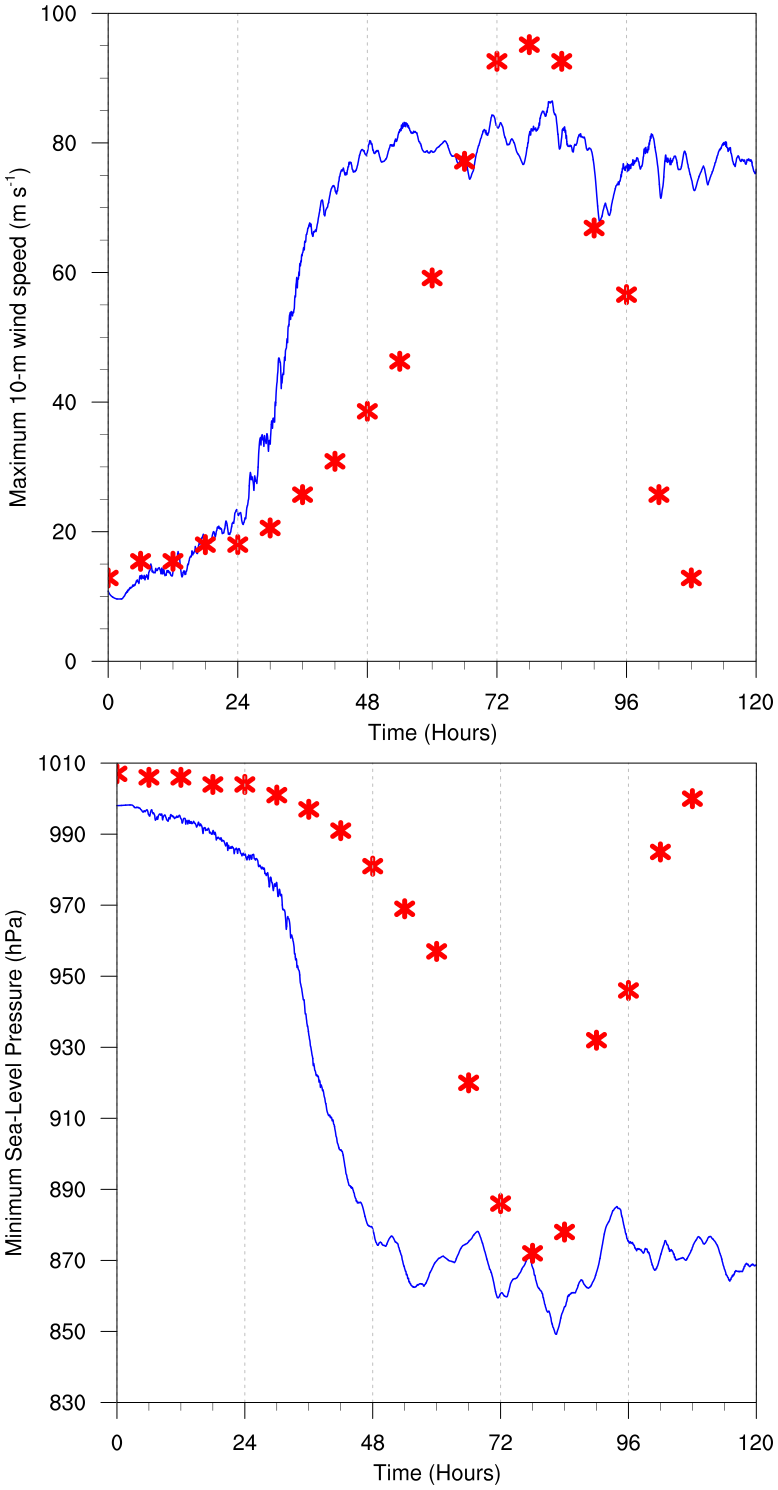
\includegraphics[width=19pc]{figures/vmax+pmin.png}}
\caption{The maximum 10-m wind speed (top panel; m s\textsuperscript{-1}) and minimum sea-level pressure (bottom panel; hPa) in the simulated storm (blue lines; plotted every minute) and from Hurricane Patricia's best track (red stars; plotted every six hours beginning at the time Patricia attained tropical storm intensity). The rapid weakening during the later stage of Patricia's lifetime was induced by landfall.}
\label{fig:vmax+pmin}
\end{figure}

%FIGURE 2%
\begin{figure}[ht]
\centerline{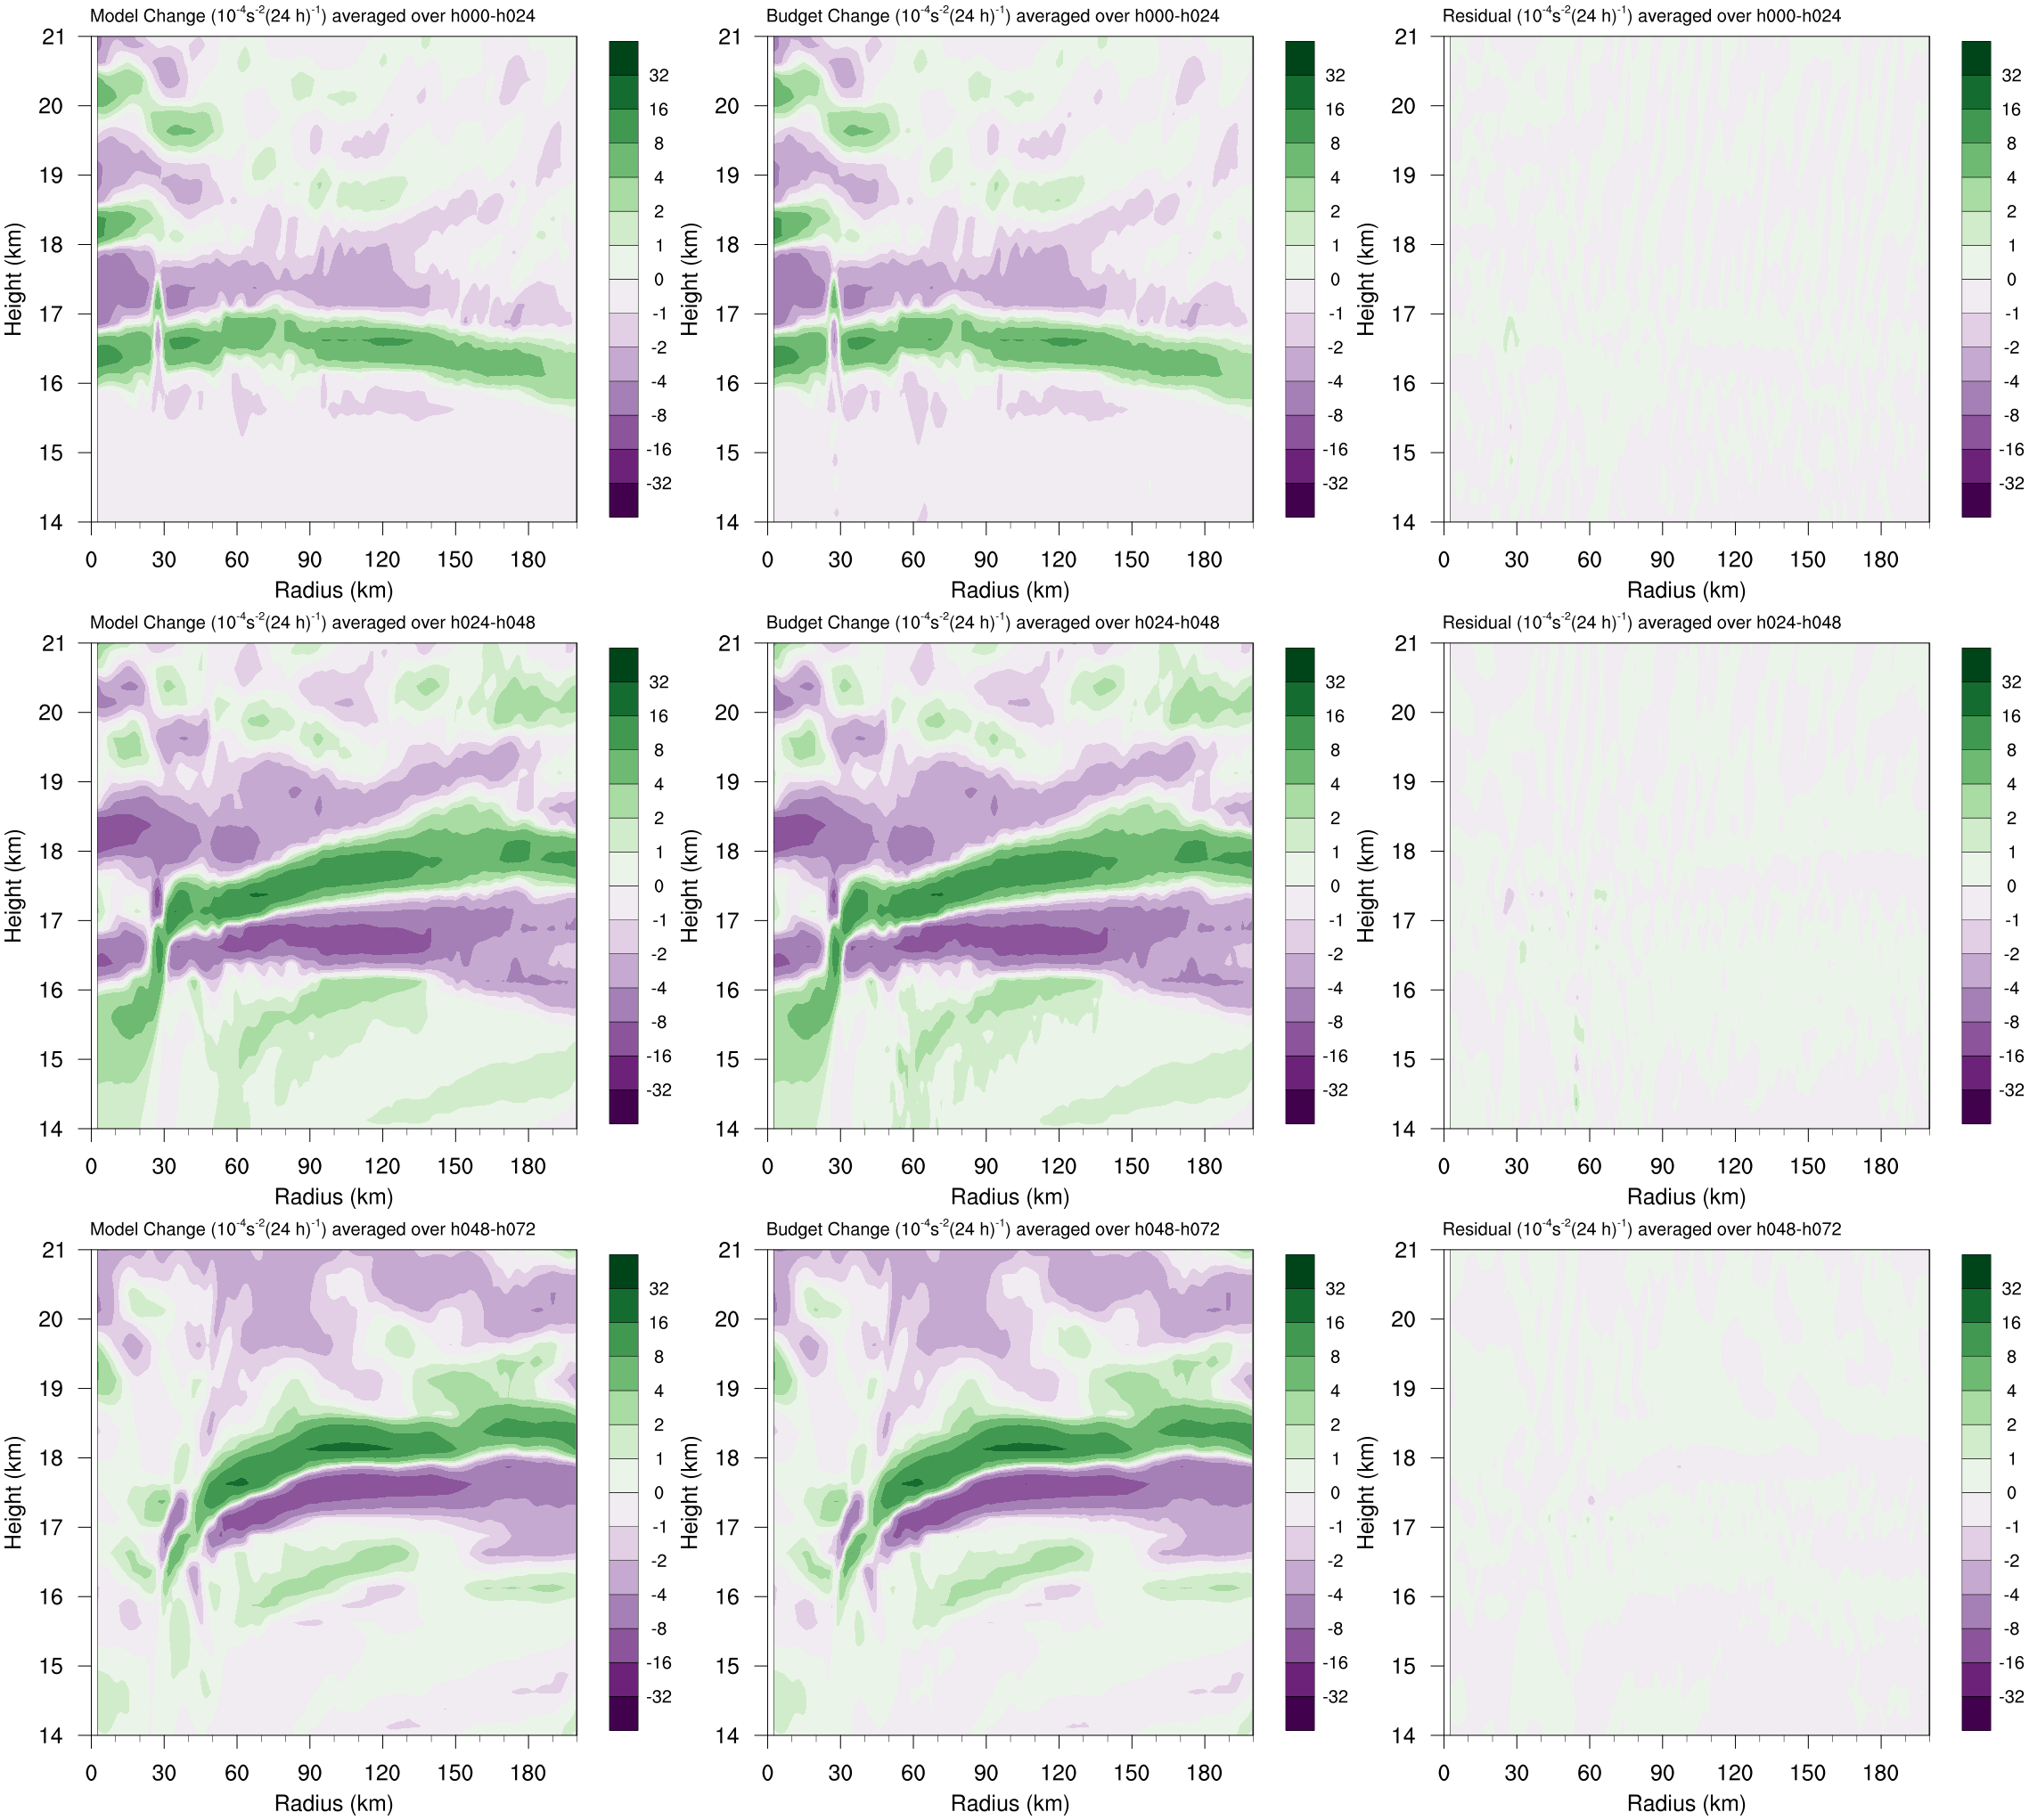
\includegraphics[width=39pc]{figures/mod+bud+res.png}}
\caption{Left panels: Twenty-four-hour changes in squared Brunt-V{\"a}is{\"a}l{\"a} frequency ($N^2$; 10\textsuperscript{-4} s\textsuperscript{-2}) computed using Eq.~\ref{eq:modelchange} over (top row) 0-24 hours, (middle row) 24-48 hours, (bottom row) 48-72 hours.
Middle Panels: The $N^2$ change over the same time periods computed using Eqs. \ref{eq:dn2dt}-\ref{eq:budgetchange}, %together with Eqs. \ref{eq:dn2dt}, \ref{eq:dthetadt}.
Right Panels: The budget residual over the same time periods, computed by subtracting the budget change (middle column) from the model change (left column).
Orange lines represent the cold-point tropopause height averaged over the same time periods.}
\label{fig:mod+bud+res}
\end{figure}

%FIGURE 3%
\begin{figure}[ht]
\centerline{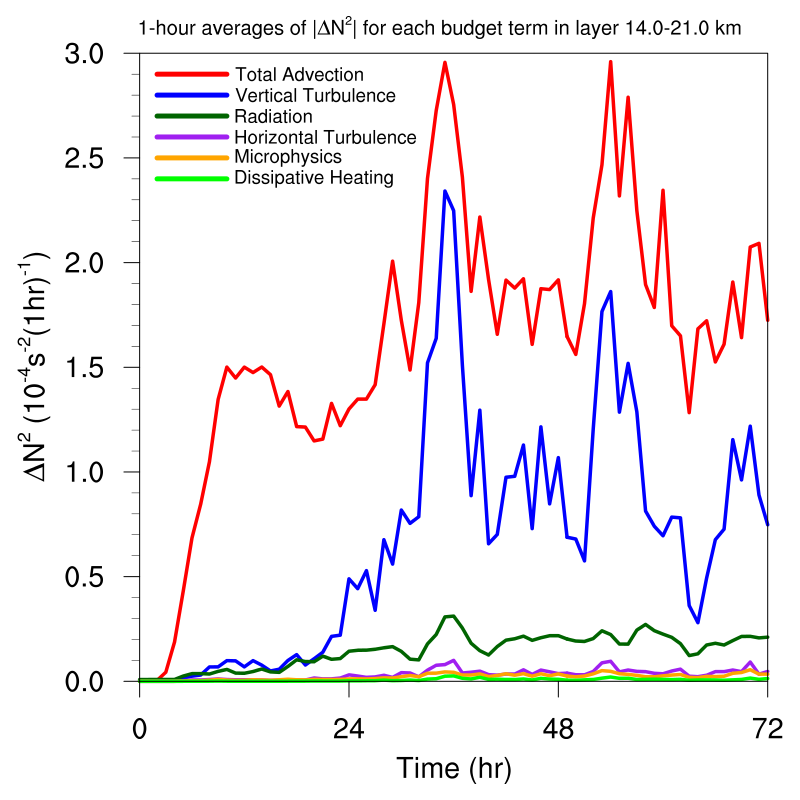
\includegraphics[width=19pc]{figures/AVG_budterms.png}}
\caption{Time series of the contribution of each of the budget terms to the time tendency of the squared Brunt-V{\"a}is{\"a}l{\"a} frequency ($N^2$; 10\textsuperscript{-4} s\textsuperscript{-2}).
For each budget term, the absolute value of the $N^2$ tendency is averaged temporally over 1-hour periods (using output every minute), and spatially in a region extending from 0 to 200 km radius and 14 to 21 km altitude.}
\label{fig:avgbudterms}
\end{figure}

%FIGURE 4%
\begin{figure*}[ht]
\centerline{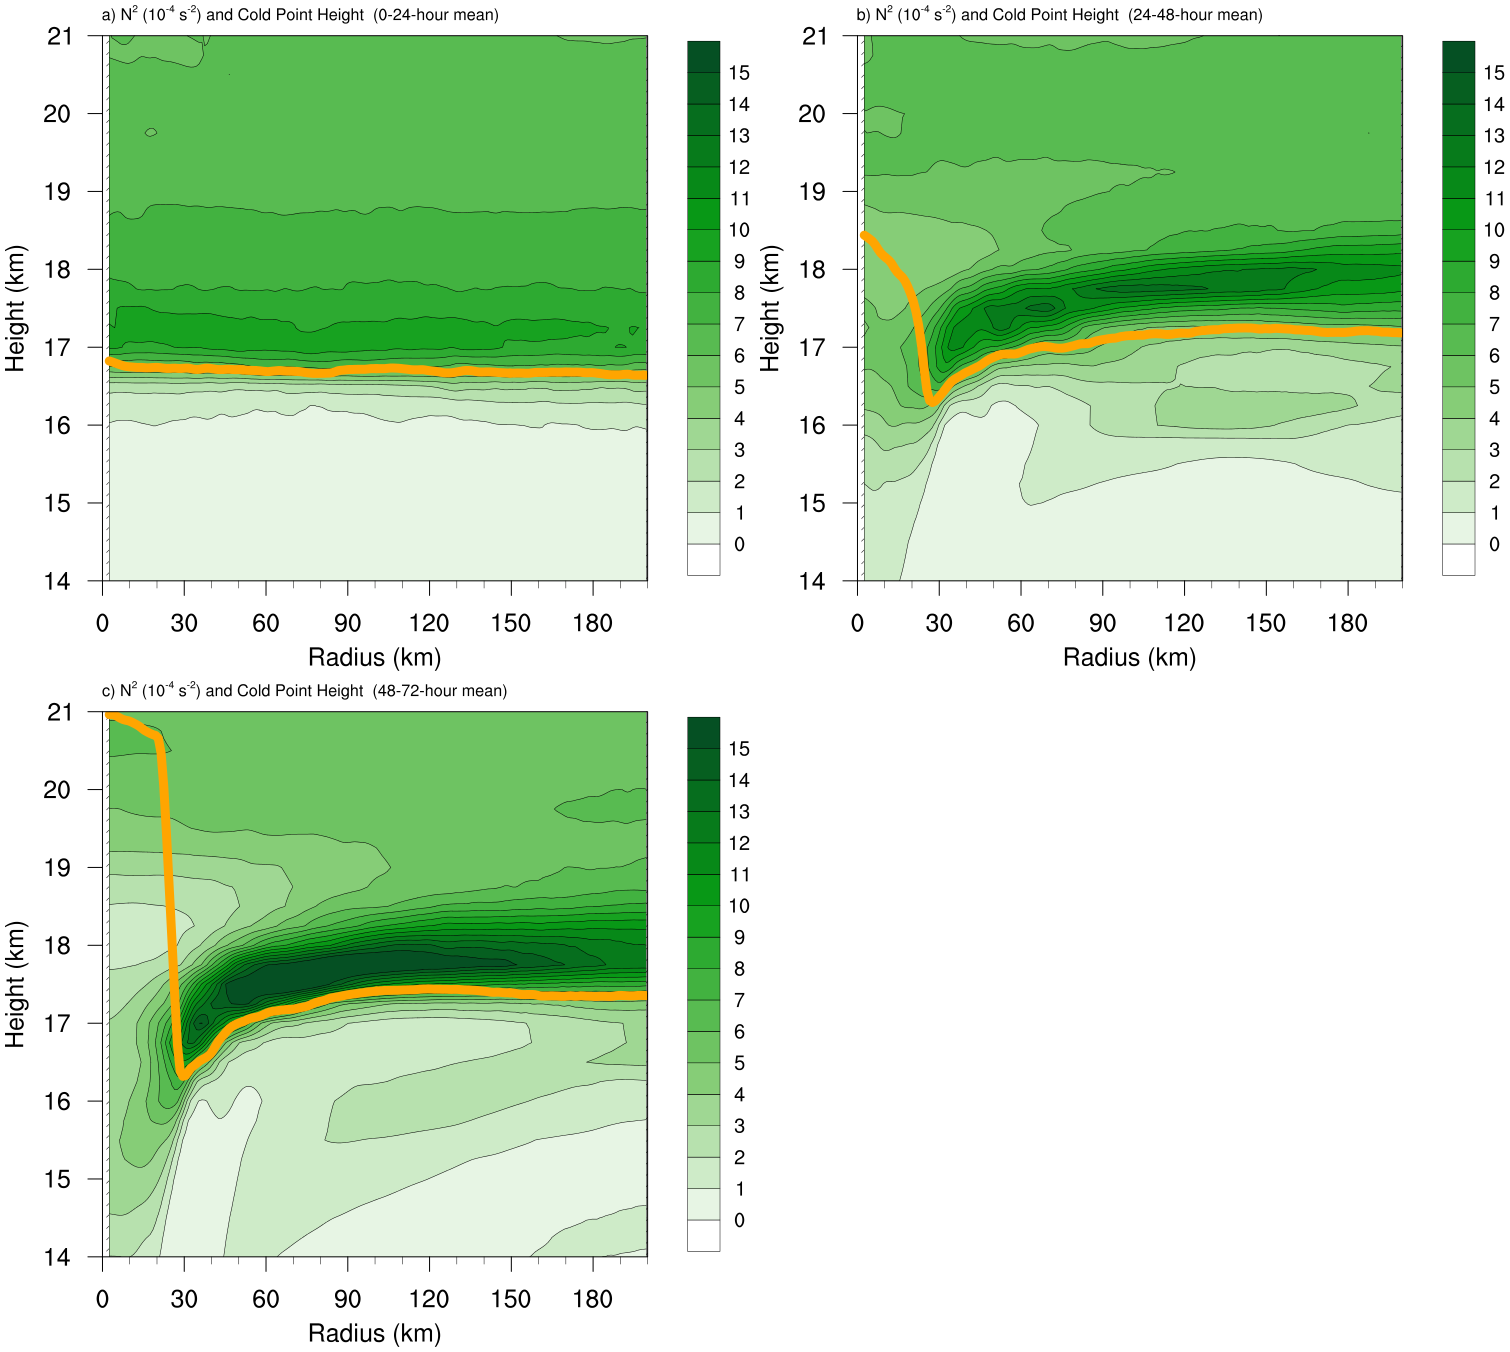
\includegraphics[width=39pc]{figures/n2-24hr-avgs.png}}
\caption{Twenty-four-hour averages of squared Brunt-V{\"a}is{\"a}l{\"a} frequency ($N^2$; 10\textsuperscript{-4} s\textsuperscript{-2}) over (a) 0-24 hours, (b) 24-48 hours, (c) 48-72 hours.
Orange lines represent the cold-point tropopause height averaged over the same time periods.}
\label{fig:n2-24hr-avgs}
\end{figure*}

%FIGURE 5%
\begin{figure*}[ht]
\centerline{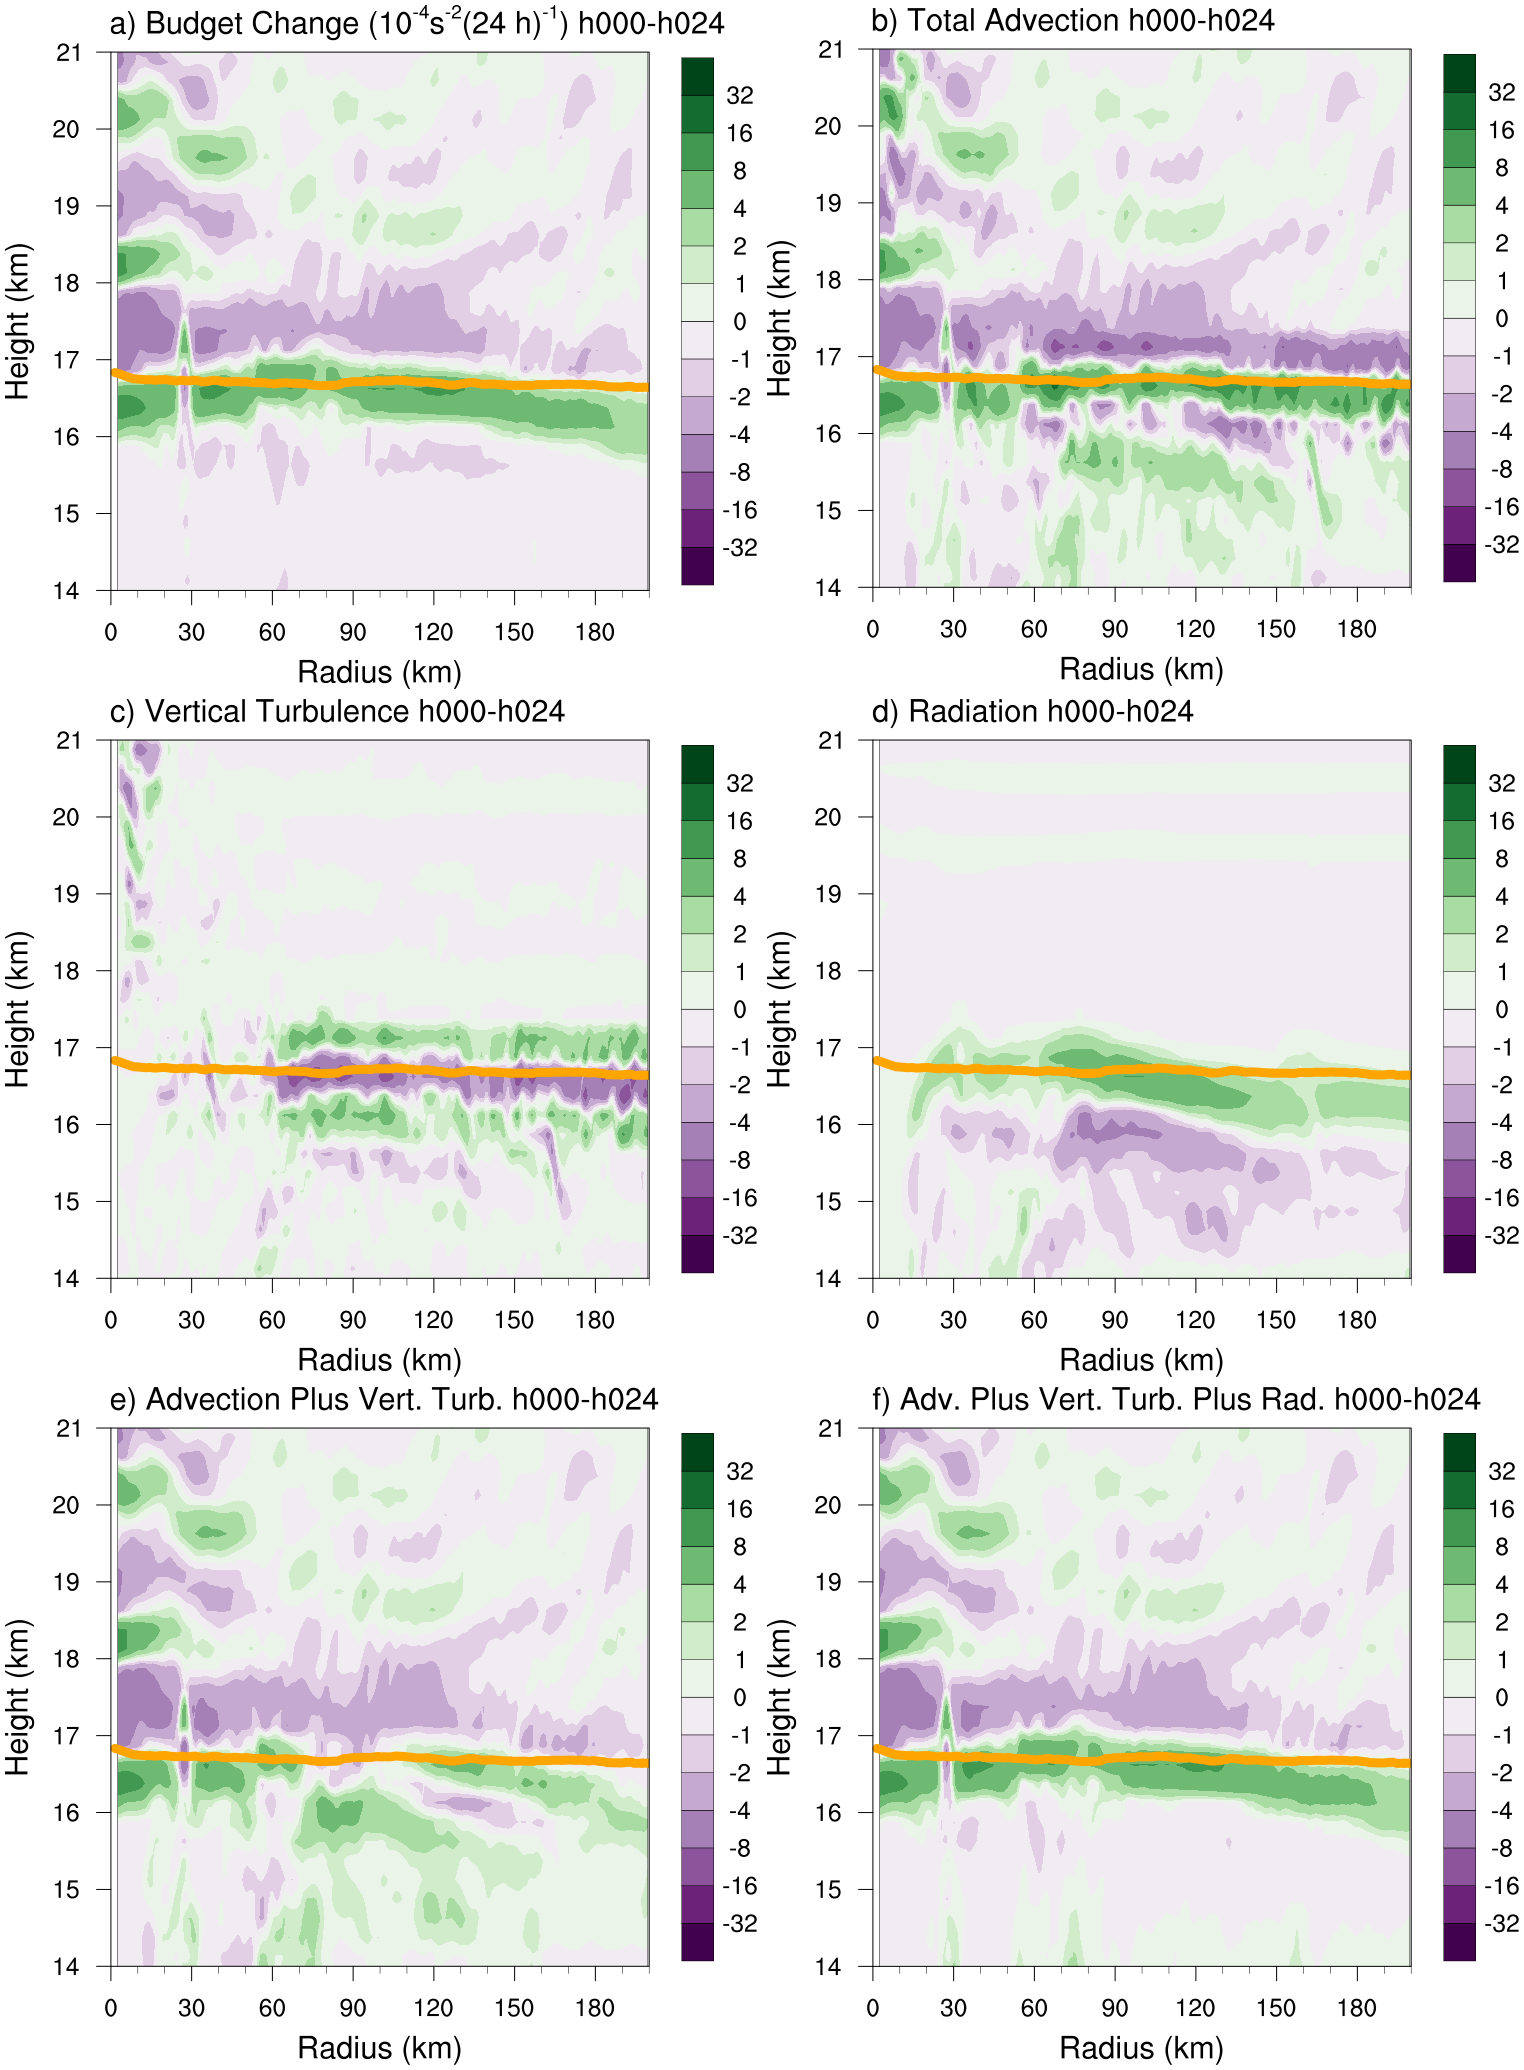
\includegraphics[width=39pc]{figures/h000-h024-budgetterms.png}}
\end{figure*}
\begin{figure}
\caption{(a) Total change in $N^2$ over the 0-24-hour period (10\textsuperscript{-4} s\textsuperscript{-2} (24 h)\textsuperscript{-1}) and the contributions to that change from (b) the sum of horizontal and vertical advection, (c) vertical turbulence, (d) longwave and shortwave radiation, (e) the sum of horizontal advection, vertical advection, and vertical turbulence, and (f) the sum of horizontal advection, vertical advection, vertical turbulence, and longwave and shortwave radiation.
Green shading indicates regions of stabilization and purple shading indicates regions of destabilization.
Orange lines represent the cold-point tropopause height averaged over the 0-24-hour period.}
\label{fig:stab-00-24}
\end{figure}

%FIGURE 6%
\begin{figure*}[ht]
\centerline{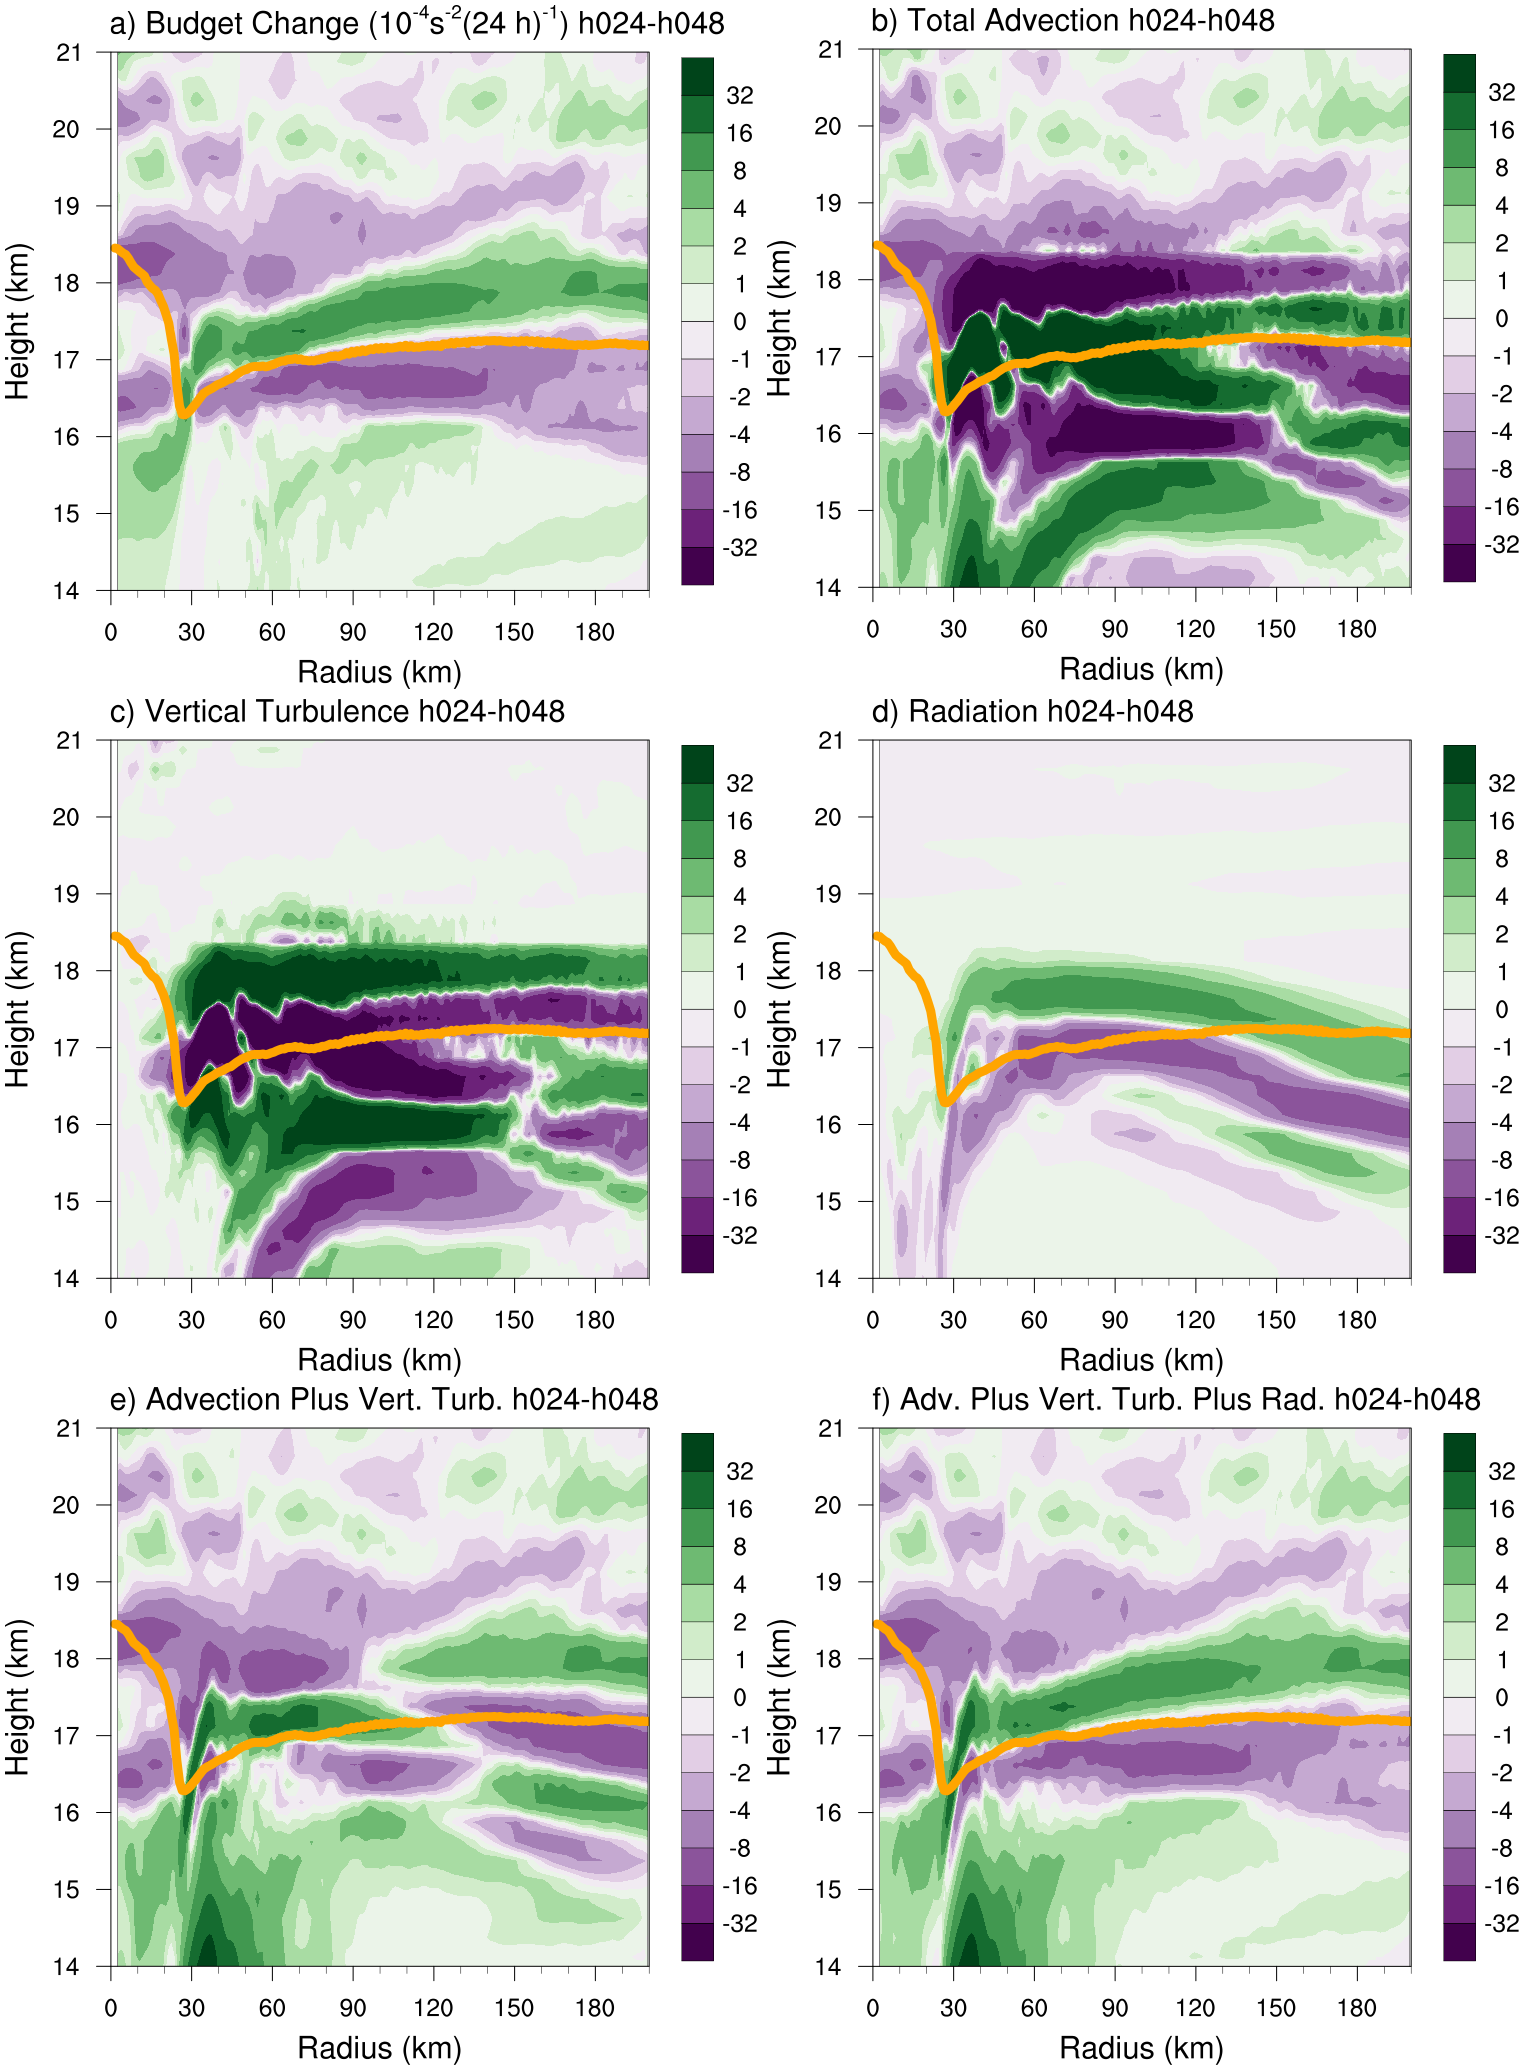
\includegraphics[width=39pc]{figures/h024-h048-budgetterms.png}}
\caption{As in Fig.~\ref{fig:stab-00-24}, but for the 24-48-hour period.}
\label{fig:stab-24-48}
\end{figure*}

%FIGURE 7%
\begin{figure*}[ht]
\centerline{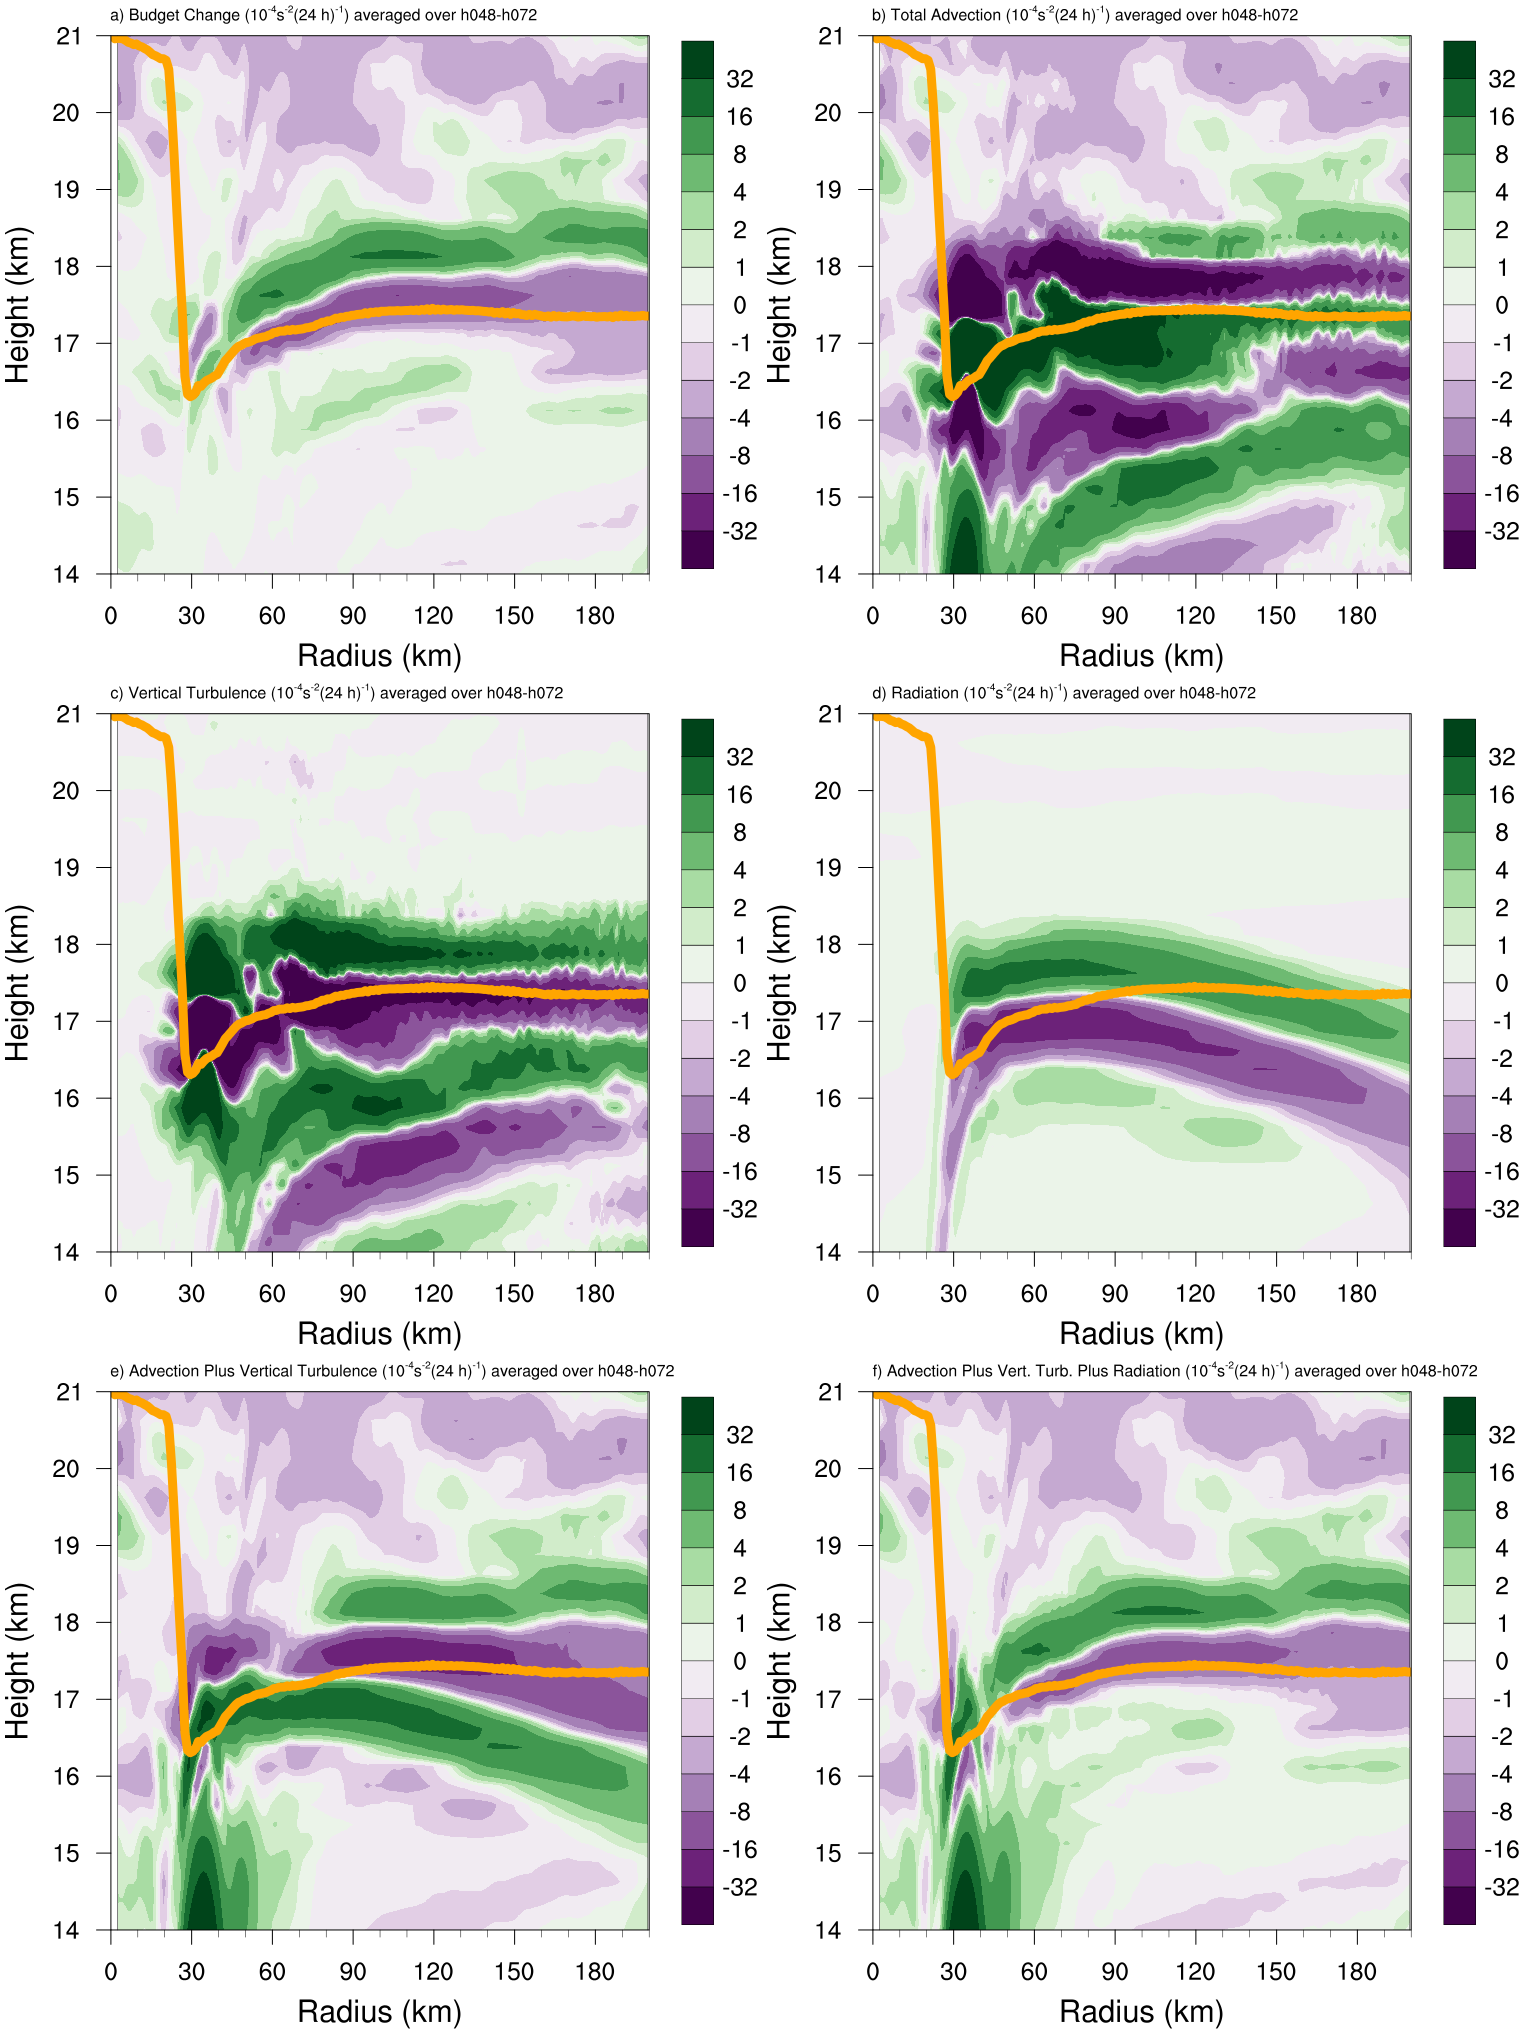
\includegraphics[width=39pc]{figures/h048-h072-budgetterms.png}}
\caption{As in Fig.~\ref{fig:stab-00-24}, but for the 48-72-hour period.}
\label{fig:stab-48-72}
\end{figure*}

%FIGURE 8%
%\begin{figure*}[ht]
%\centerline{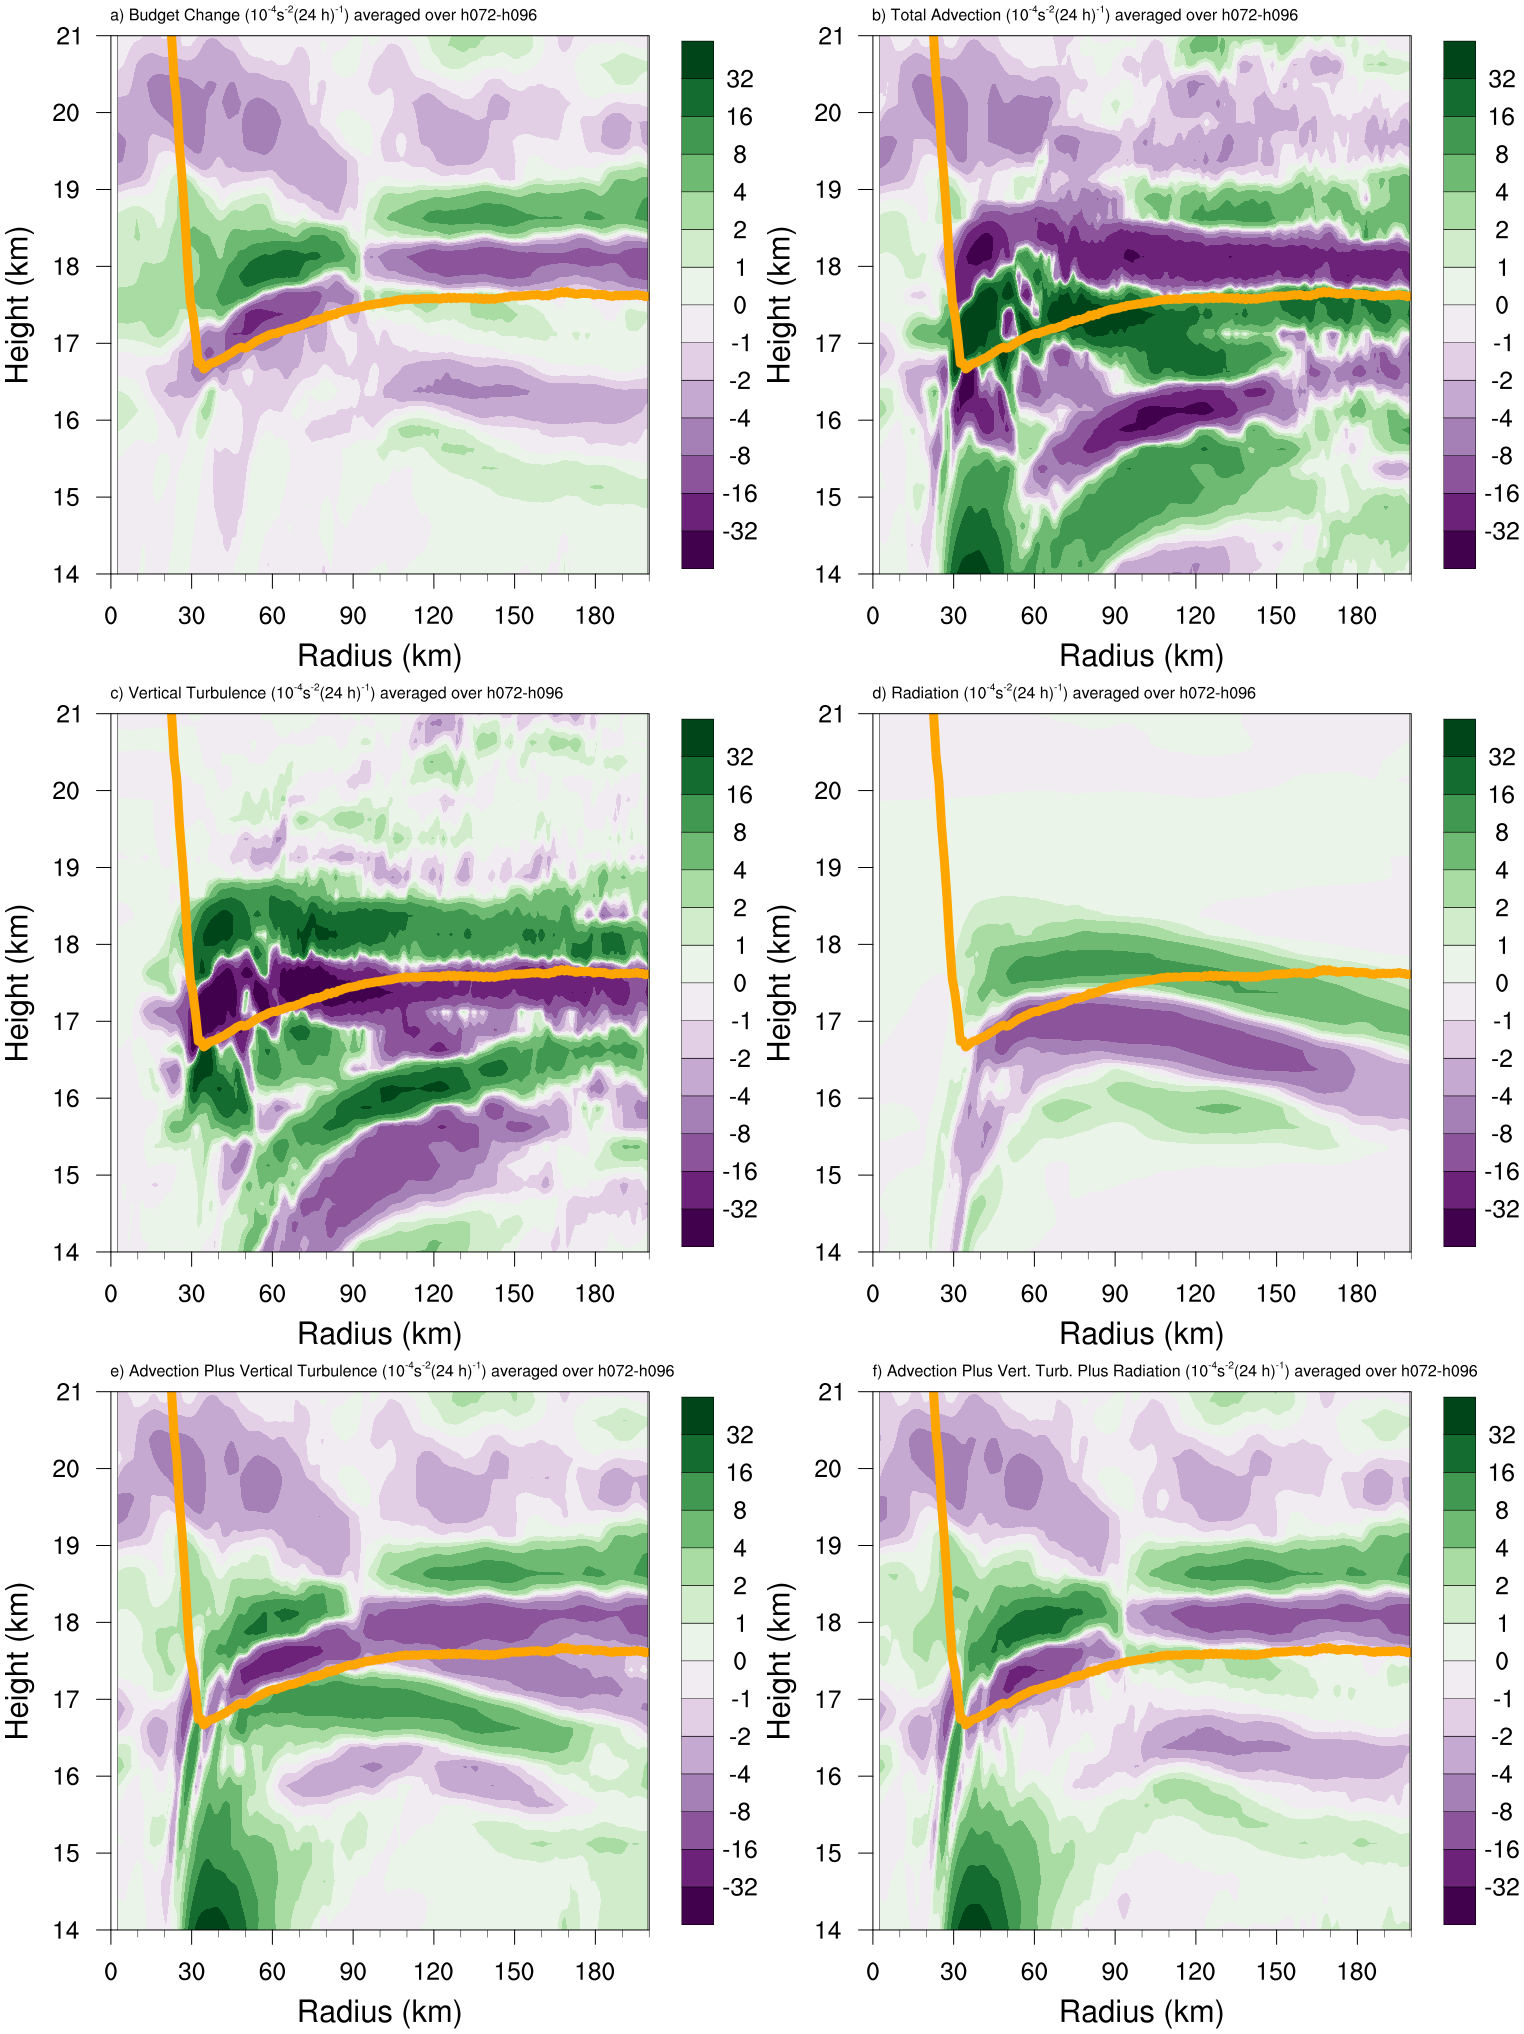
\includegraphics[width=33pc]{figures/h072-h096-budgetterms.png}}
%\caption{As in Fig.~\ref{fig:stab-48-72}, but for the 72-96-hour period.}
%\label{fig:stab-72-96}
%\end{figure*}

%FIGURE 8%
%\begin{figure*}[ht]
%\centerline{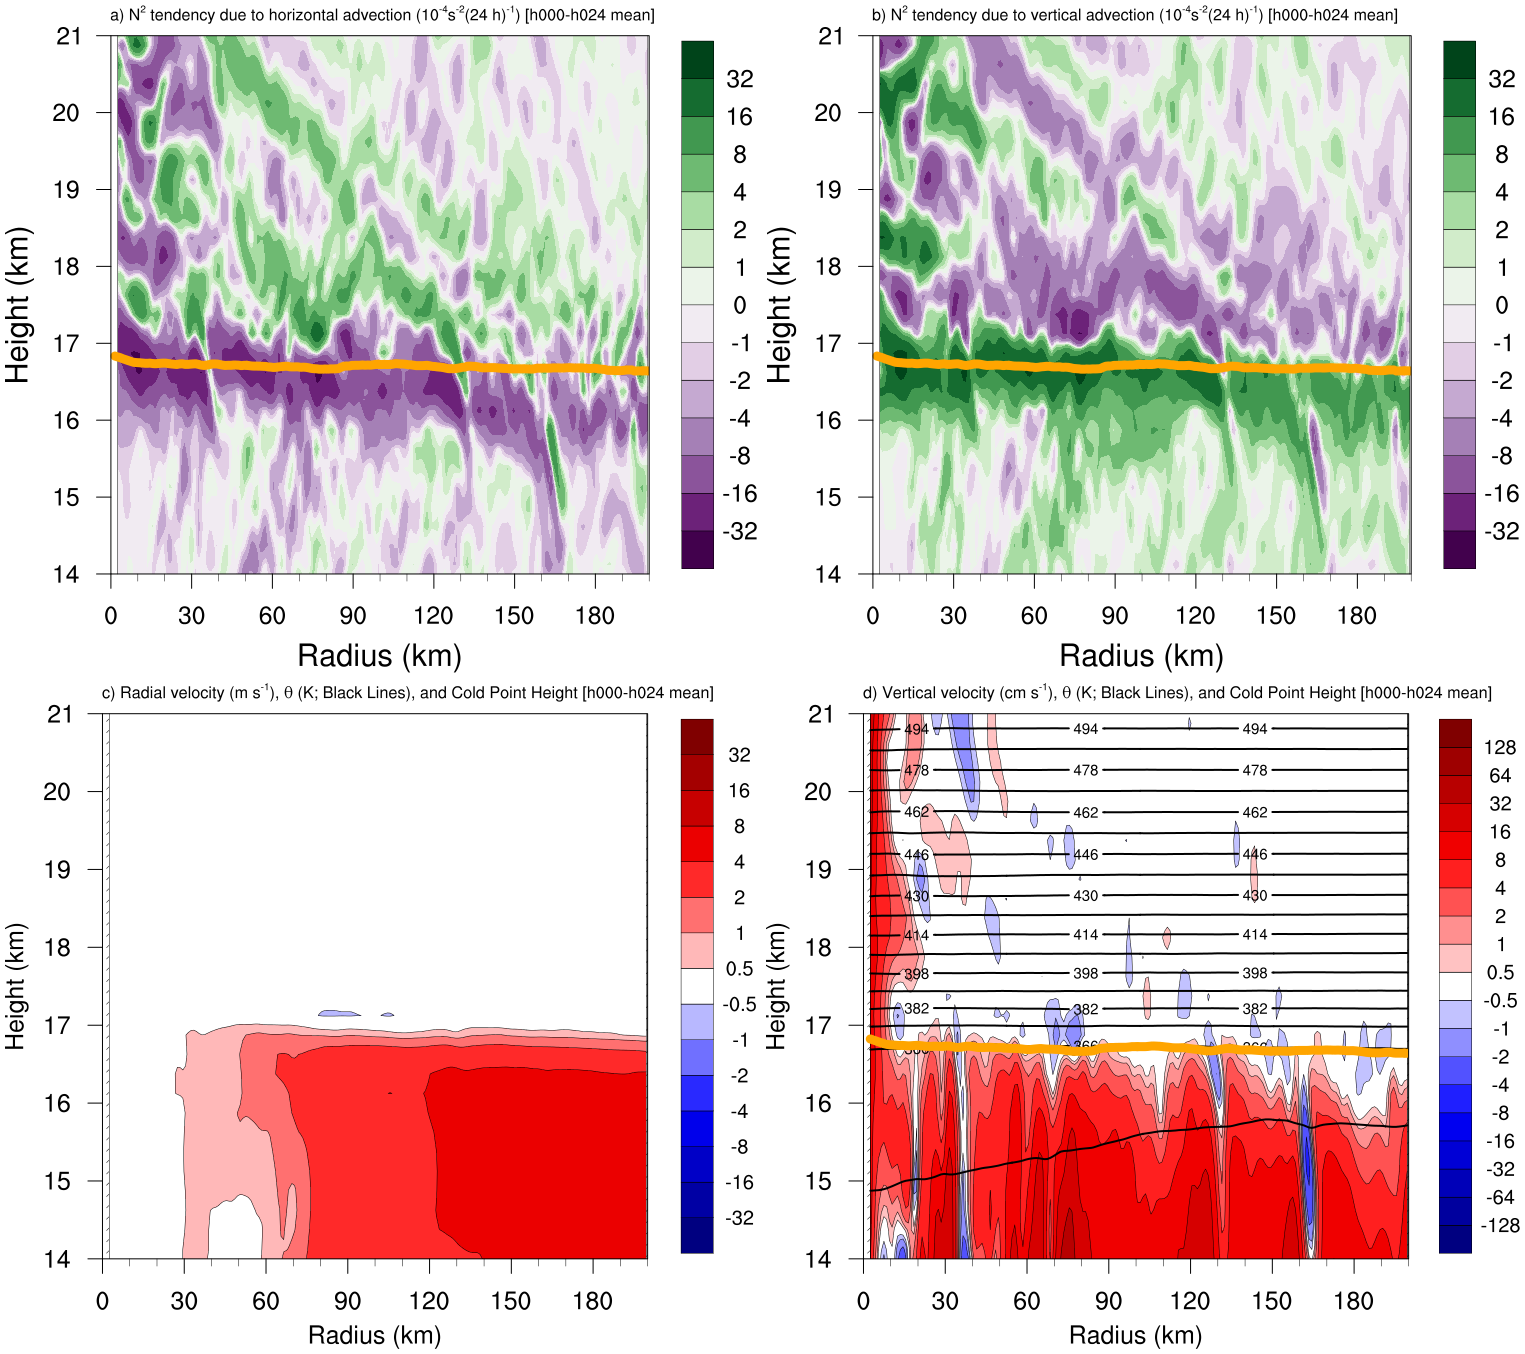
\includegraphics[width=39pc]{figures/h000-h024-adv.png}}
%\caption{The contribution to the change in $N^2$ over the 0-24-hour period (10\textsuperscript{-4} s\textsuperscript{-2} (24 hr)\textsuperscript{-1}) by (a) horizontal advection and (b) vertical advection. (c) The radial velocity (m s\textsuperscript{-1}; filled contours), potential temperature (K; thick black contours), and cold-point tropopause height (orange line) averaged over the 0-24-hour period. (d) The vertical velocity (cm s\textsuperscript{-1}; filled contours), potential temperature (K; thick black contours), and cold-point tropopause height (orange line) averaged over the 0-24-hour period.}
%\label{fig:adv-00-24}
%\end{figure*}


%FIGURE 8%
%\begin{figure*}[ht]
%\centerline{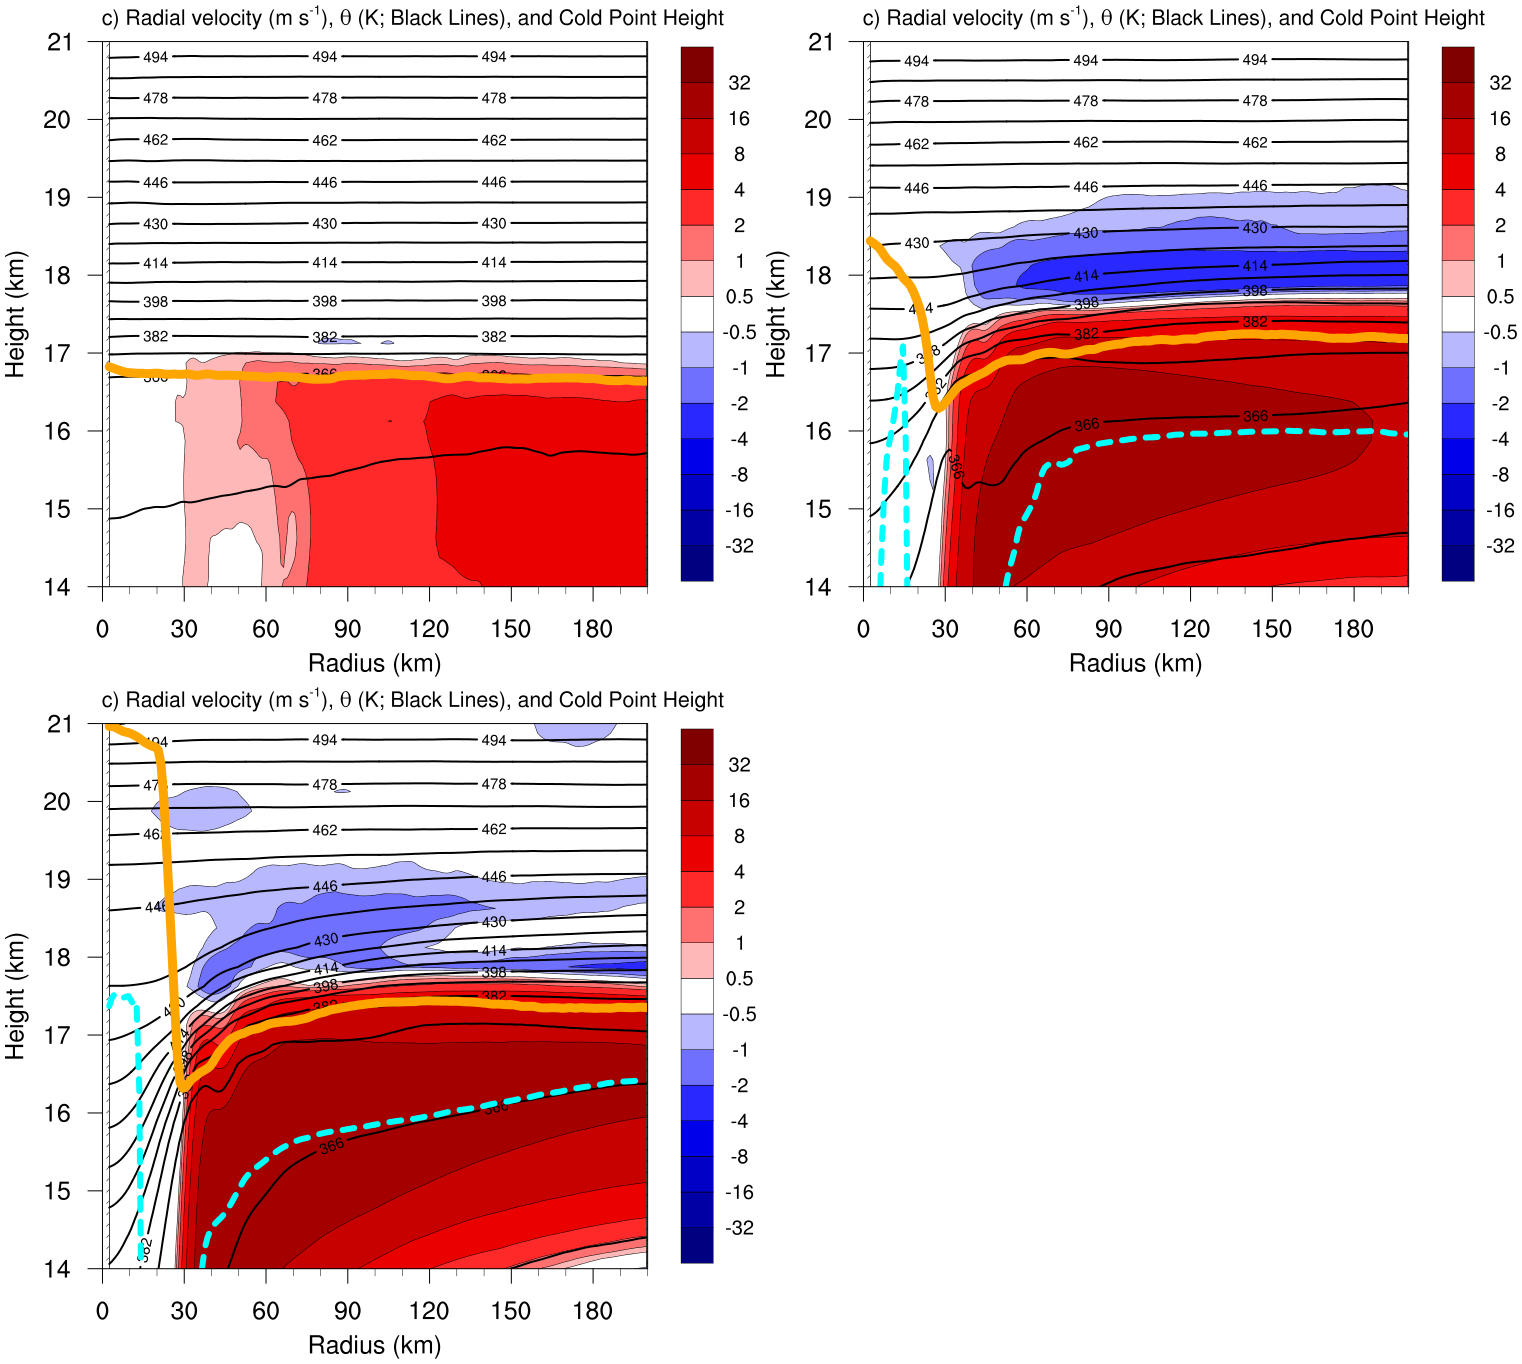
\includegraphics[width=39pc]{figures/u.png}}
%\caption{Radial velocity (m s\textsuperscript{-1}; filled contours), potential temperature (K; thick black contours), and cold-point tropopause height (orange lines) averaged over (a) 0-24 hours, (b) 24-48 hours, and (c) 48-72 hours.}
%\label{fig:u}
%\end{figure*}

%FIGURE 8%
\begin{figure*}[ht]
\centerline{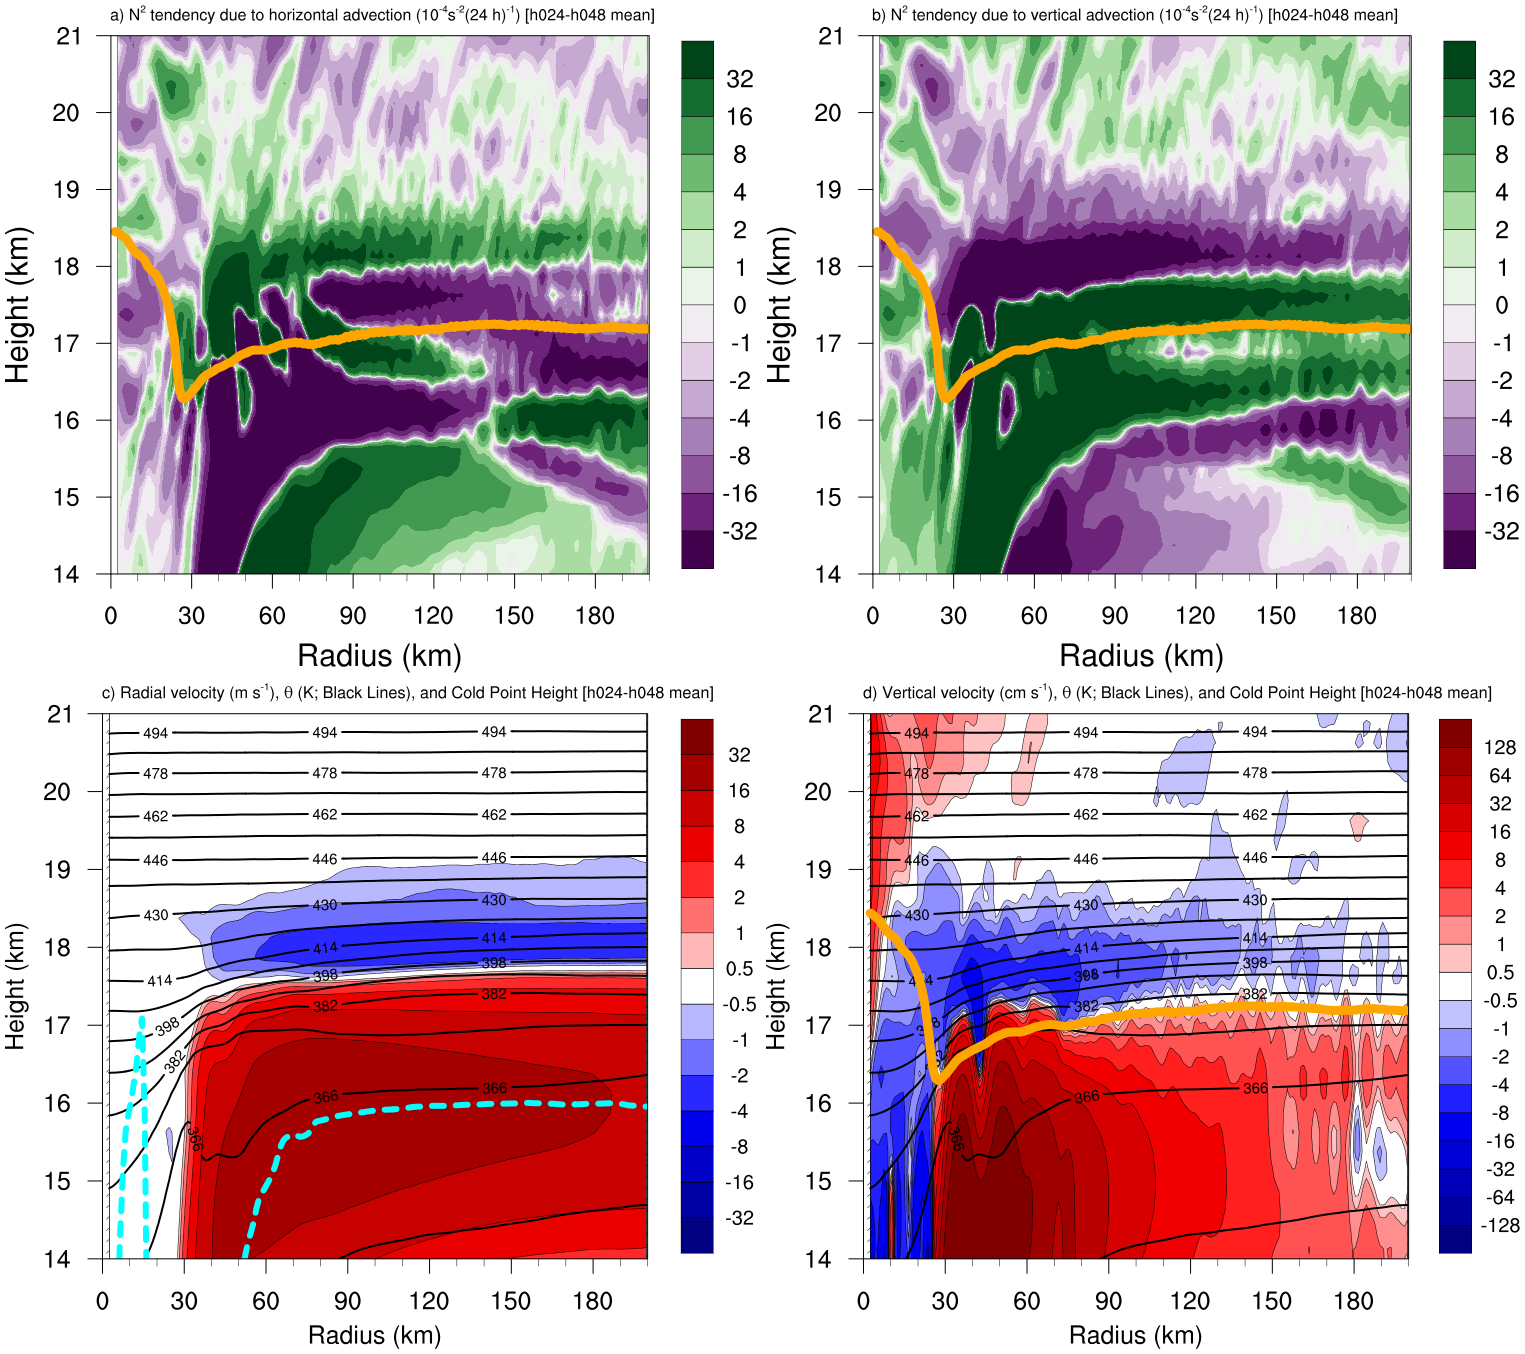
\includegraphics[width=39pc]{figures/h024-h048-adv.png}}
\caption{The contributions to the change in $N^2$ over the 24-48-hour period (10\textsuperscript{-4} s\textsuperscript{-2} (24 h)\textsuperscript{-1}) by (a) horizontal advection and (b) vertical advection. (c) The radial velocity (m s\textsuperscript{-1}; filled contours), potential temperature (K; thick black contours), cold-point tropopause height (orange line), and level of maximum outflow (dashed cyan line) averaged over the 24-48-hour period. (d) The vertical velocity (cm s\textsuperscript{-1}; filled contours), potential temperature (K; thick black contours), and cold-point tropopause height (orange line) averaged over the 24-48-hour period.}
%\caption{As in Fig. \ref{fig:adv-00-24}, but for the 24-48-hour period.}
\label{fig:adv-24-48}
\end{figure*}

%FIGURE 9%
%\begin{figure*}[ht]
%\centerline{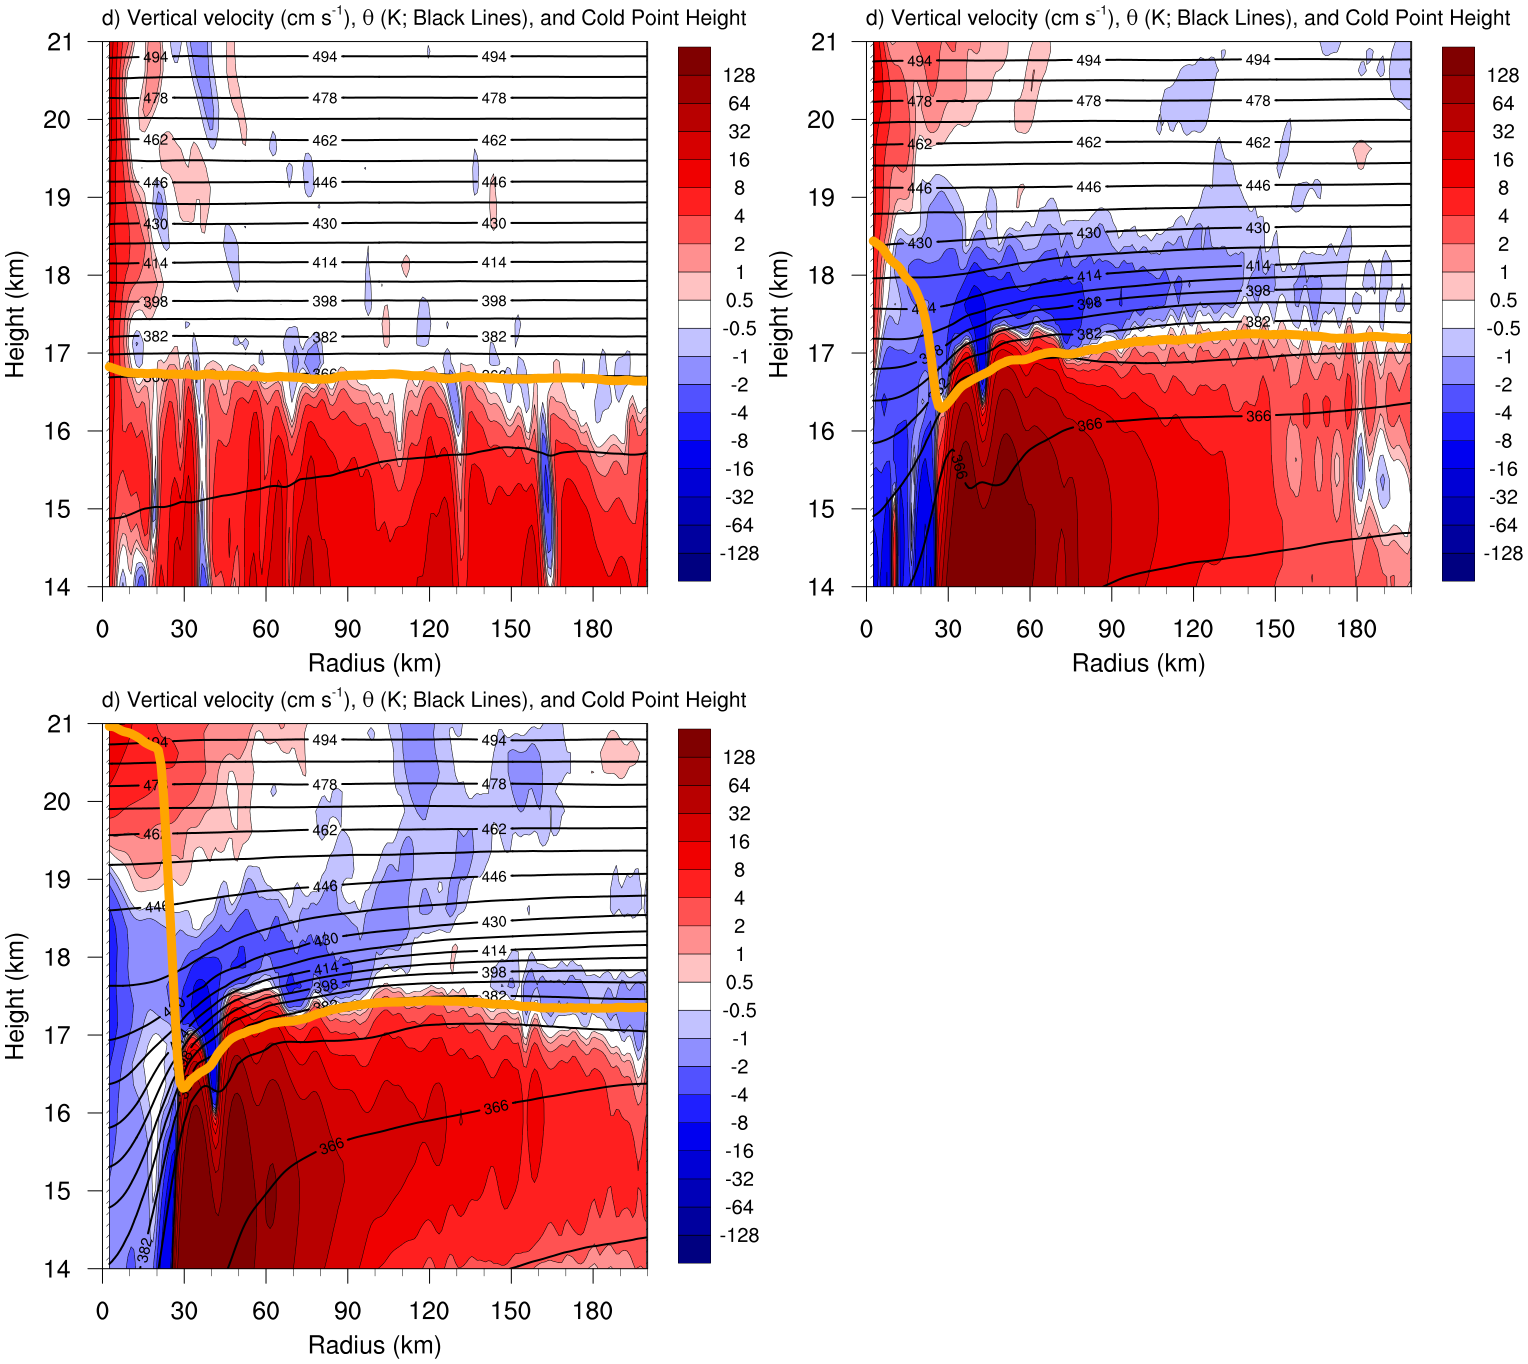
\includegraphics[width=39pc]{figures/w.png}}
%\caption{Vertical velocity (cm s\textsuperscript{-1}; filled contours), potential temperature (K; thick black contours), and cold-point tropopause height (orange lines) averaged over (a) 0-24 hours, (b) 24-48 hours, and (c) 48-72 hours.}
%\label{fig:w}
%\end{figure*}

%FIGURE 10%
%\begin{figure*}[ht]
%\centerline{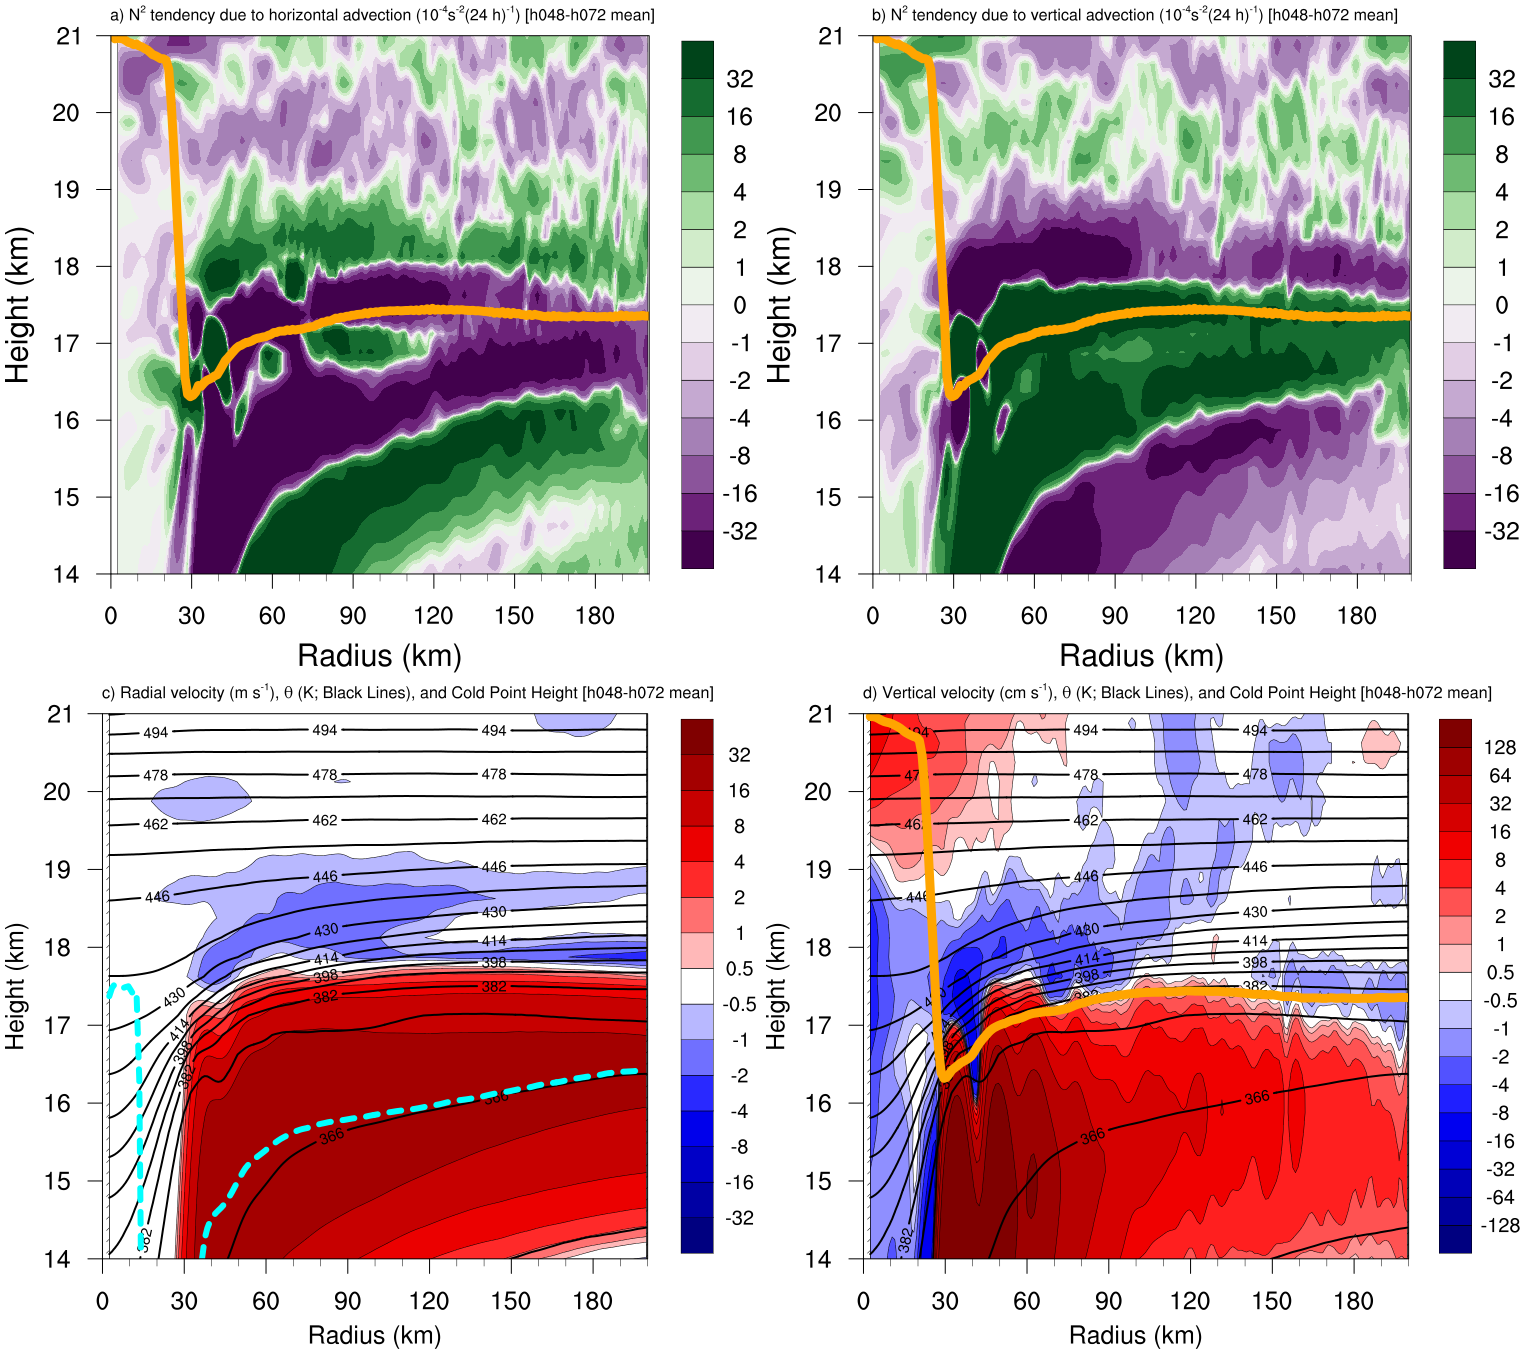
\includegraphics[width=39pc]{figures/h048-h072-adv.png}}
%\caption{As in Fig. \ref{fig:adv-00-24}, but for the 48-72-hour period.}
%\label{fig:adv-48-72}
%\end{figure*}

%FIGURE 9%
\begin{figure*}[ht]
\centerline{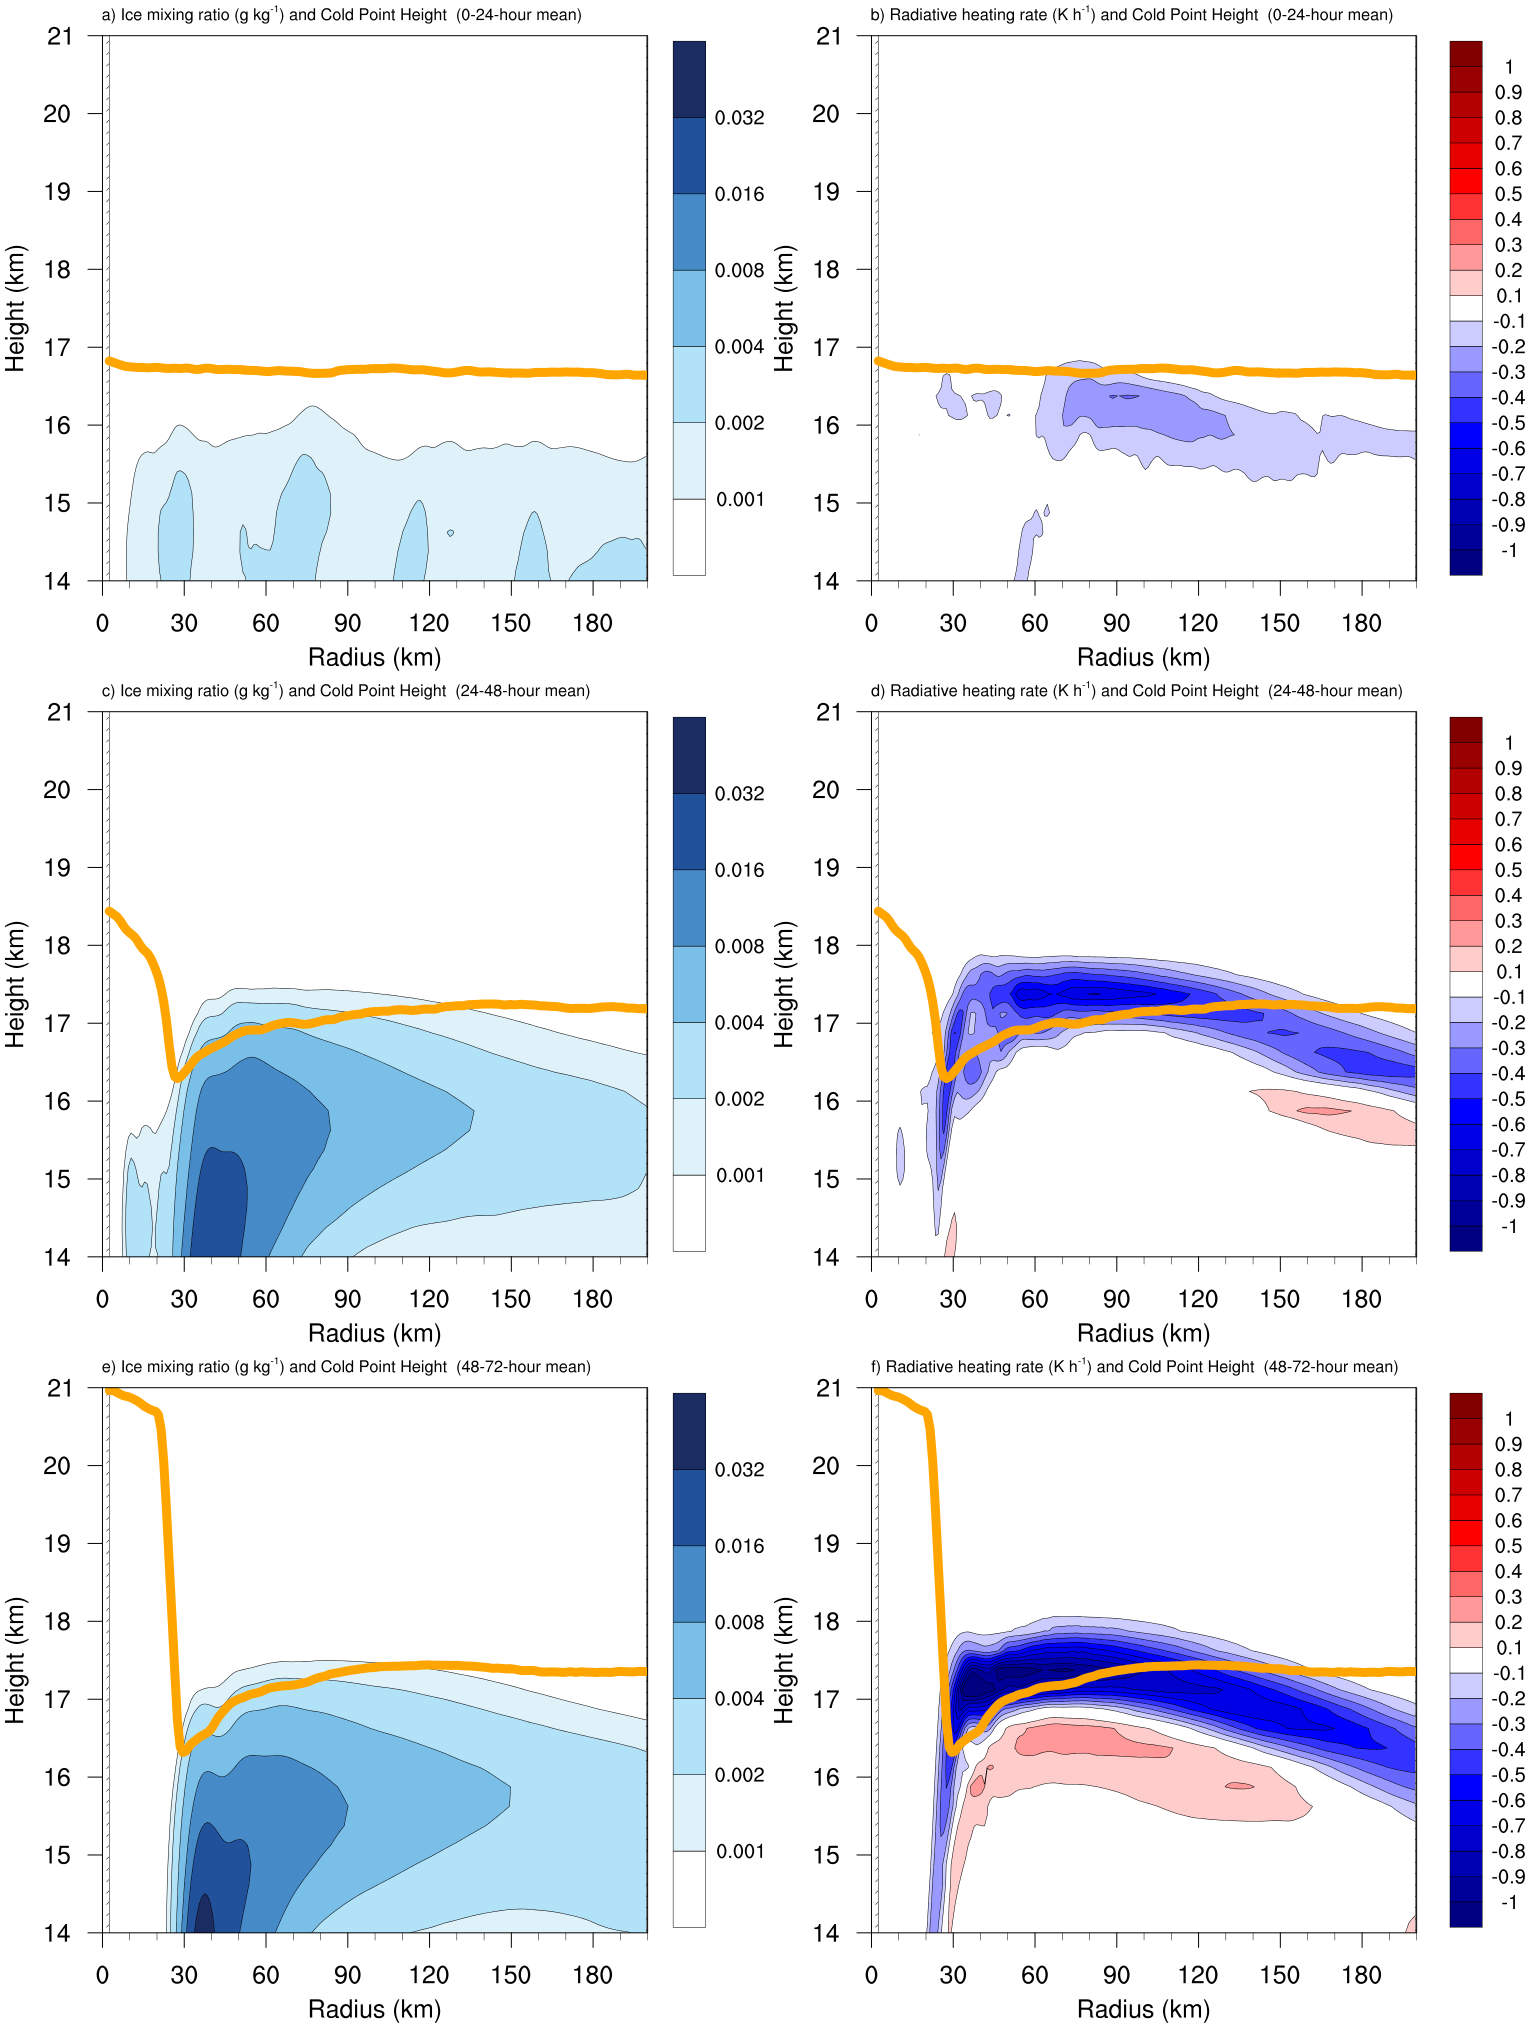
\includegraphics[width=39pc]{figures/qi+radten.png}}
\end{figure*}
\begin{figure}
\caption{Ice mixing ratio (g kg\textsuperscript{-1}) and cold-point tropopause height (orange lines) averaged over (a) 0-24 hours, (c) 24-48 hours, and (e) 48-72 hours. Radiative heating rate (K h\textsuperscript{-1}) and cold-point tropopause height (orange lines) averaged over (b) 0-24 hours, (d) 24-48 hours, and (f) 48-72 hours.} 
\label{fig:qi+radten}
\end{figure}

%FIGURE 10%
\begin{figure*}[ht]
\centerline{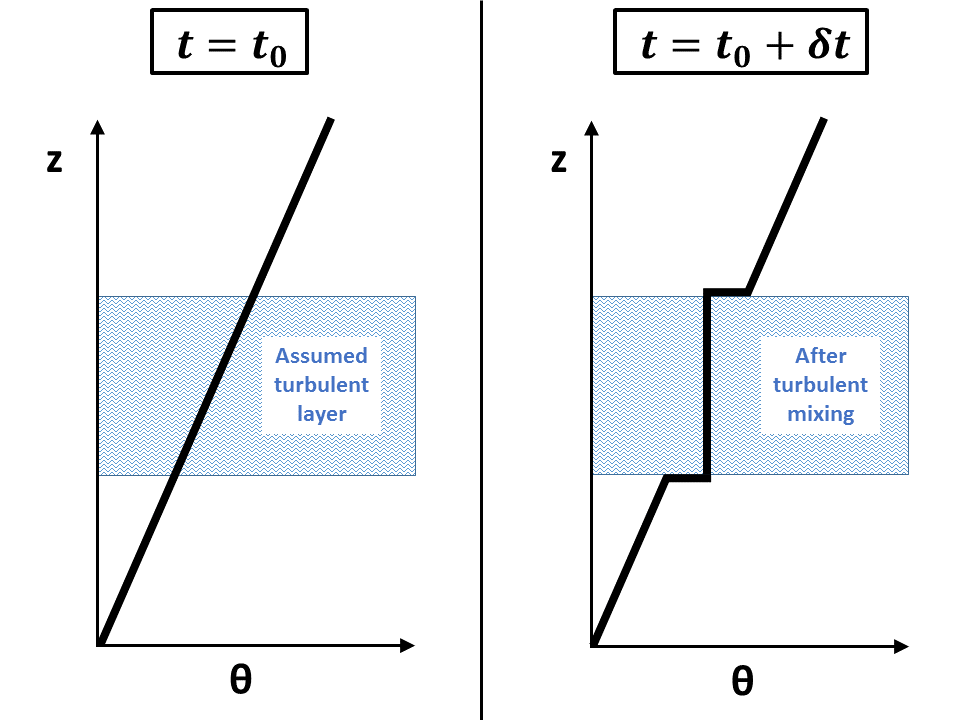
\includegraphics[width=39pc]{figures/Schematic2.png}}
   \caption{Schematic diagram of the effect of turbulent mixing on the vertical profile of potential temperature ($\theta$). At the initial time (left panel), potential temperature is assumed to increase with height at a constant rate (thick black line). The imposition of turbulence within a portion of the layer (blue hatching) adjusts the potential temperature profile toward the mean initial value of that layer. After a period of mixing (right panel) the potential temperature in the mixed layer does not vary with height, but just above and just below the mixed layer, it rapidly increases with height.}
\label{fig:schematic}
\end{figure*}

%FIGURE 11%
\begin{figure*}[ht]
\centerline{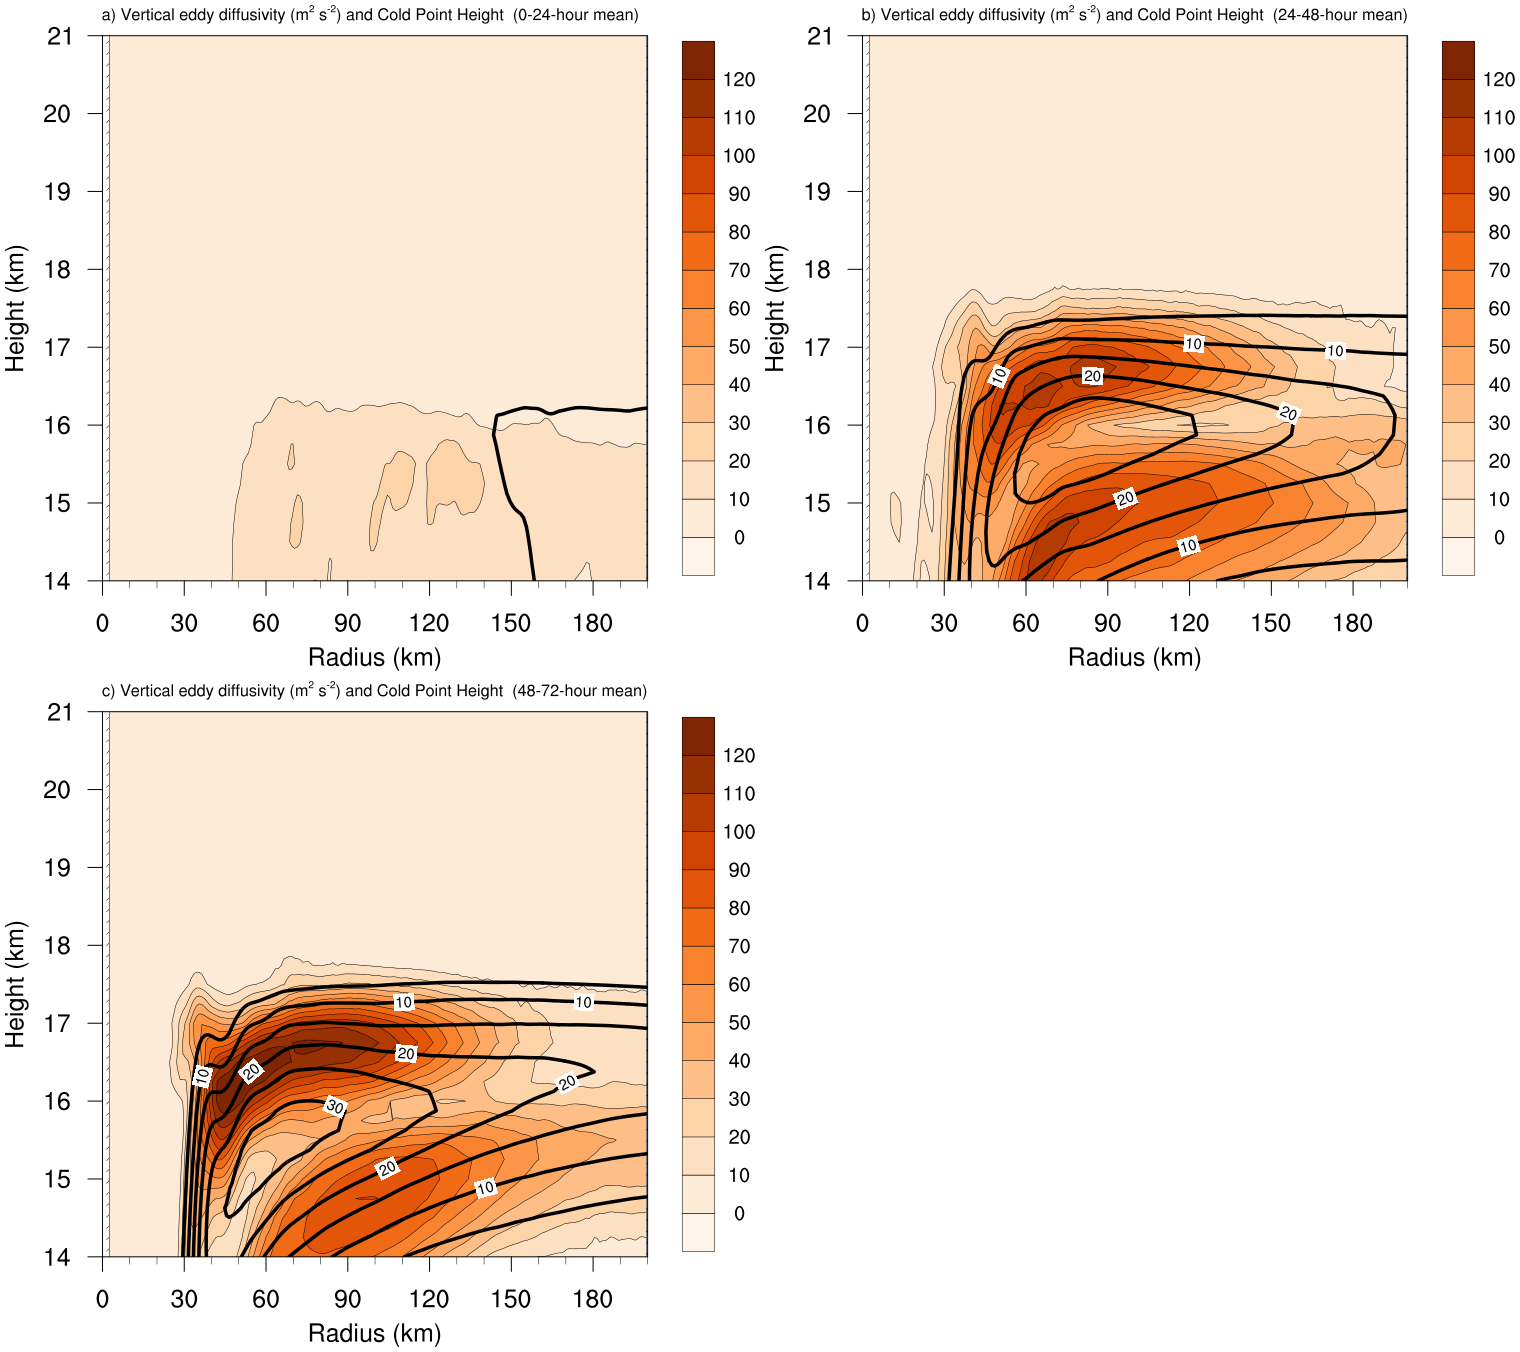
\includegraphics[width=39pc]{figures/khvten.png}}
\caption{Vertical eddy diffusivity (m\textsuperscript{2} s\textsuperscript{-2}; filled contours), cold-point tropopause height (cyan lines), and radial velocity (m s\textsuperscript{-1}; thick black lines) averaged over (a) 0-24 hours, (b) 24-48 hours, and (c) 48-72 hours.}
\label{fig:diff}
\end{figure*}

%FIGURE 12%
\begin{figure*}[ht]
\centerline{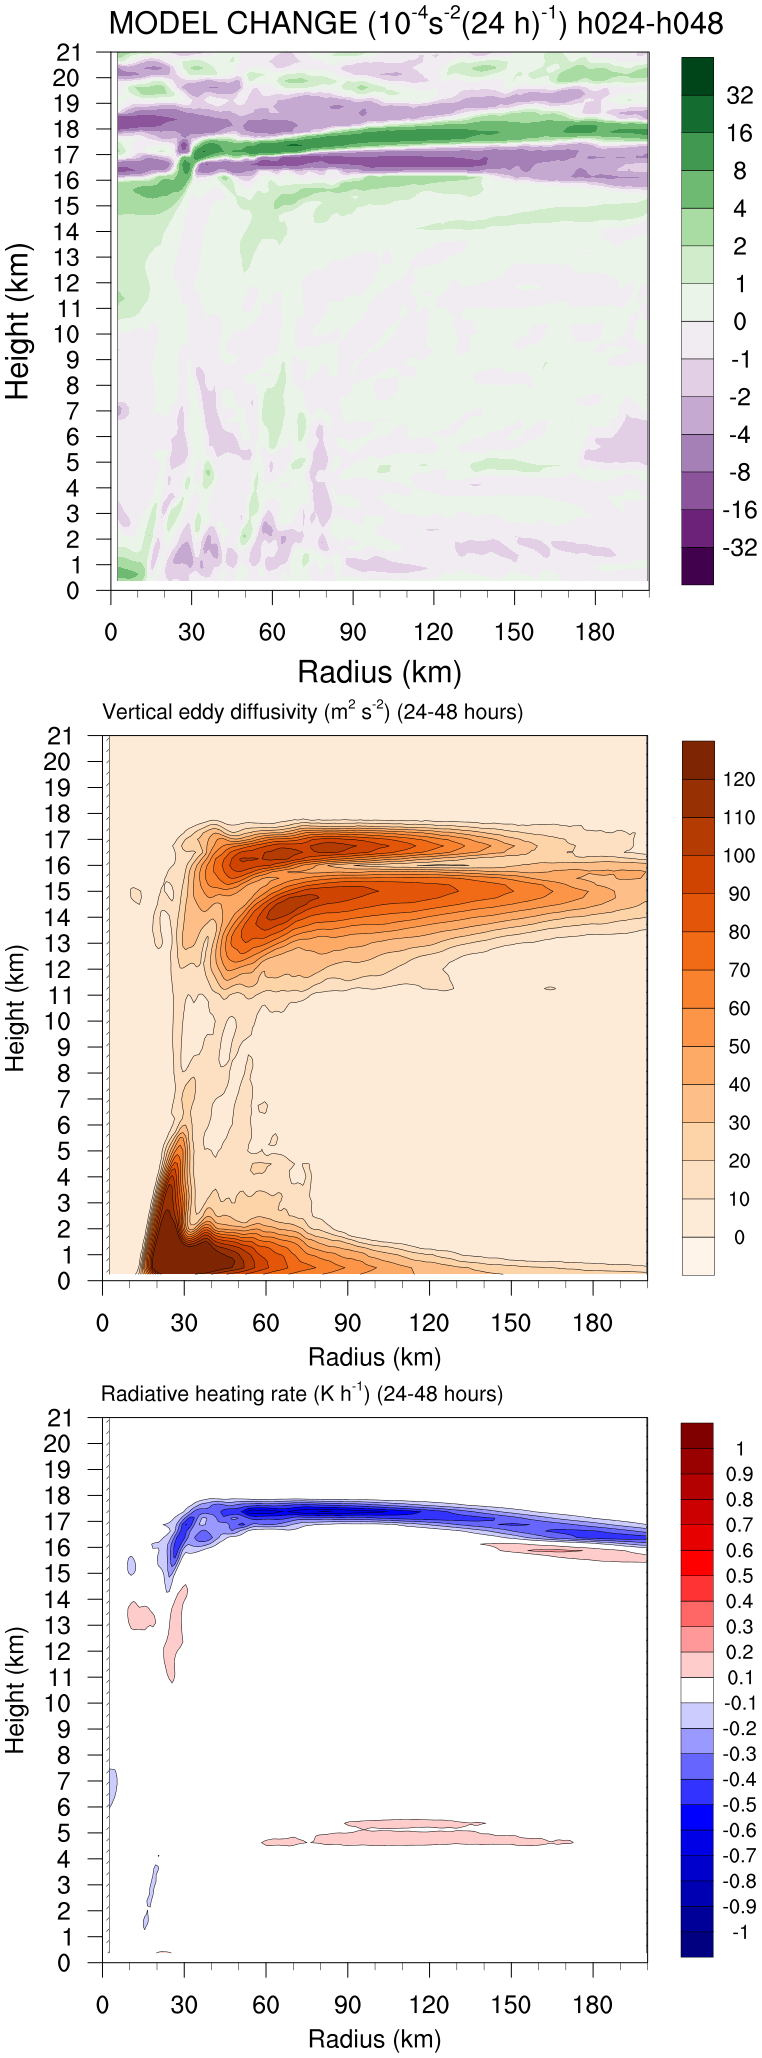
\includegraphics[width=19pc]{figures/fulltrop.png}}
\end{figure*}
\begin{figure}
\caption{(Top panel) Change in $N^2$ over the 24-48-hour period (10\textsuperscript{-4} s\textsuperscript{-2} (24 h)\textsuperscript{-1}) directly output by the model for the 0-21-km layer. (Middle panel) Vertical eddy diffusivity (m\textsuperscript{2} s\textsuperscript{-2}) averaged over the same time period. (Bottom panel) Radiative heating rate (K h\textsuperscript{-1}) averaged over the same time period.}
\label{fig:fulltrop}
\end{figure}

%%FIGURE A1%
%\begin{figure*}[ht]
%\centerline{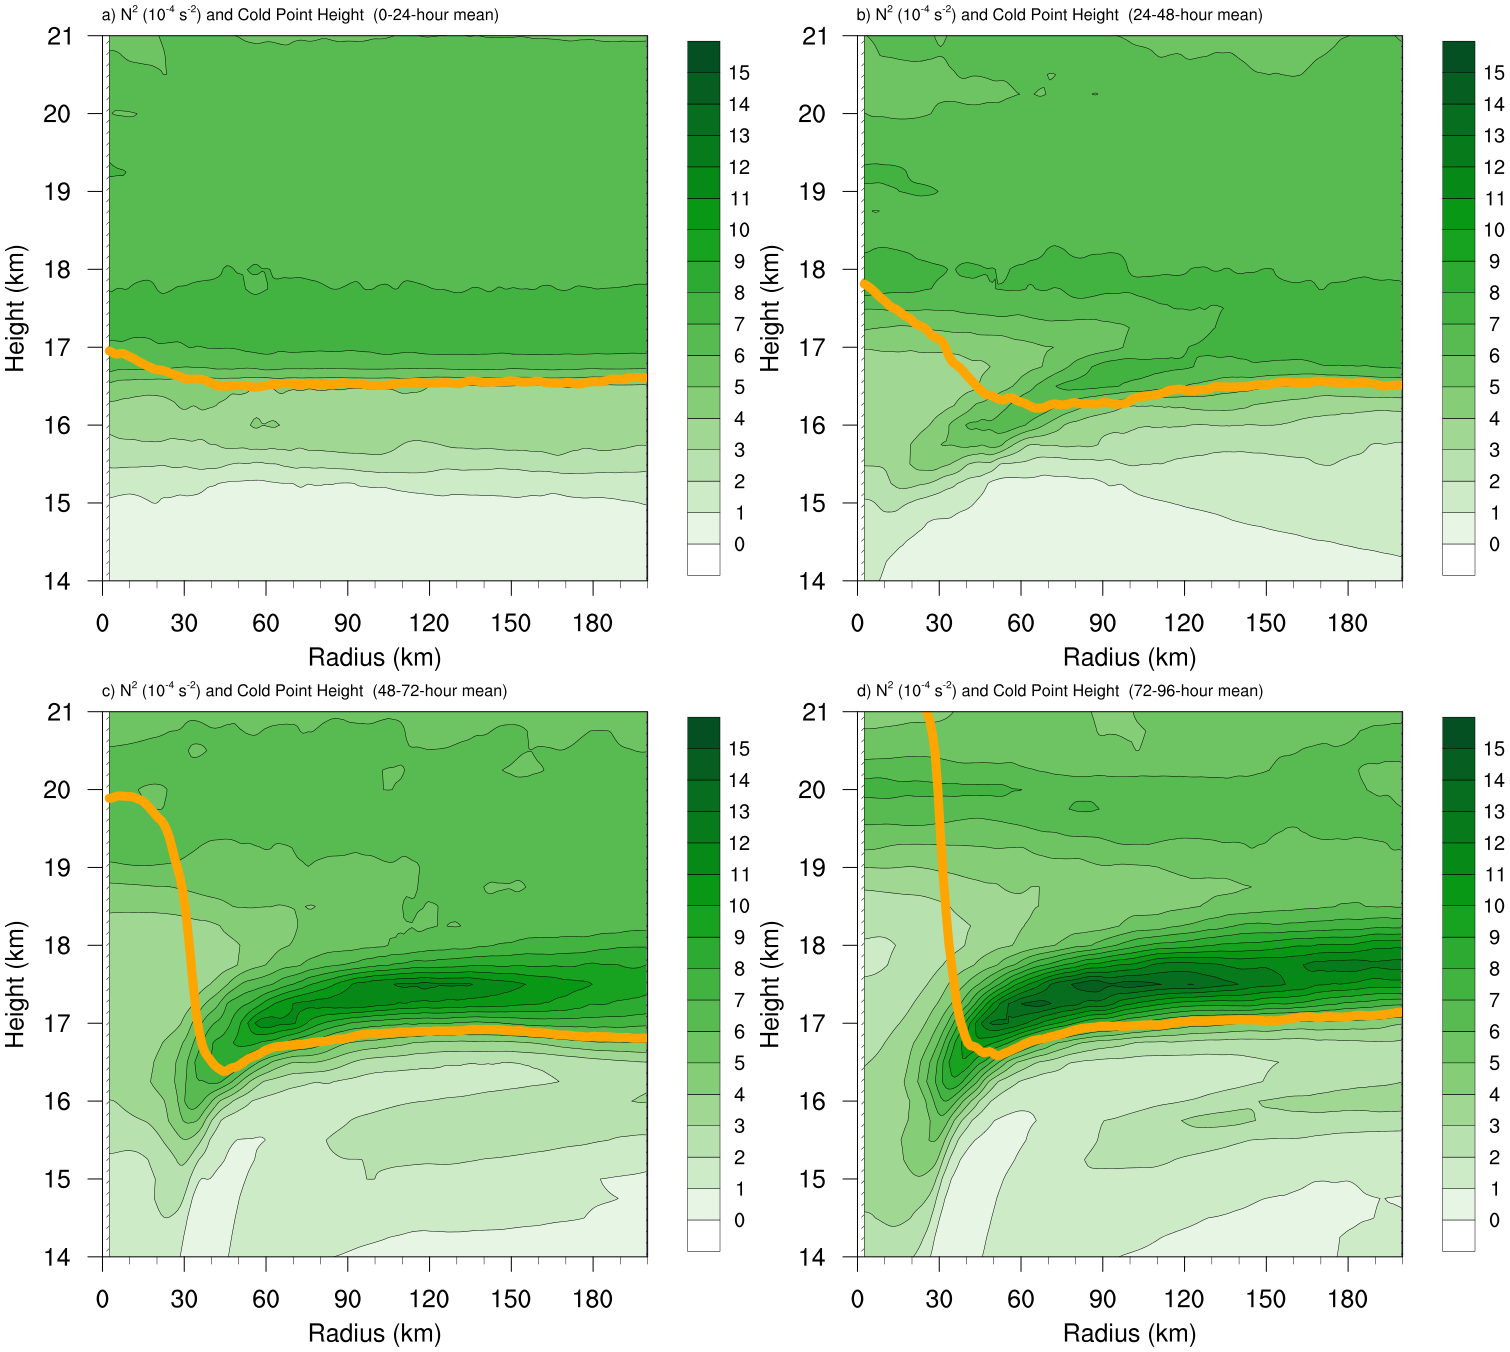
\includegraphics[width=39pc]{figures/n2-1000km.png}}
%\appendcaption{A1}{Twenty-four-hour averages of squared Brunt-V{\"a}is{\"a}l{\"a} frequency ($N^2$; 10\textsuperscript{-4} s\textsuperscript{-2}) over (a) 0-24 hours, (b) 24-48 hours, (c) 48-72 hours, and (d) 72-96 hours for the simulation described in Appendix Aa. Orange lines represent the cold-point tropopause height averaged over the same time periods.}
%\label{fig:n2-1000km}
%\end{figure*}
%
%%FIGURE A2%
%\begin{figure*}[ht]
%\centerline{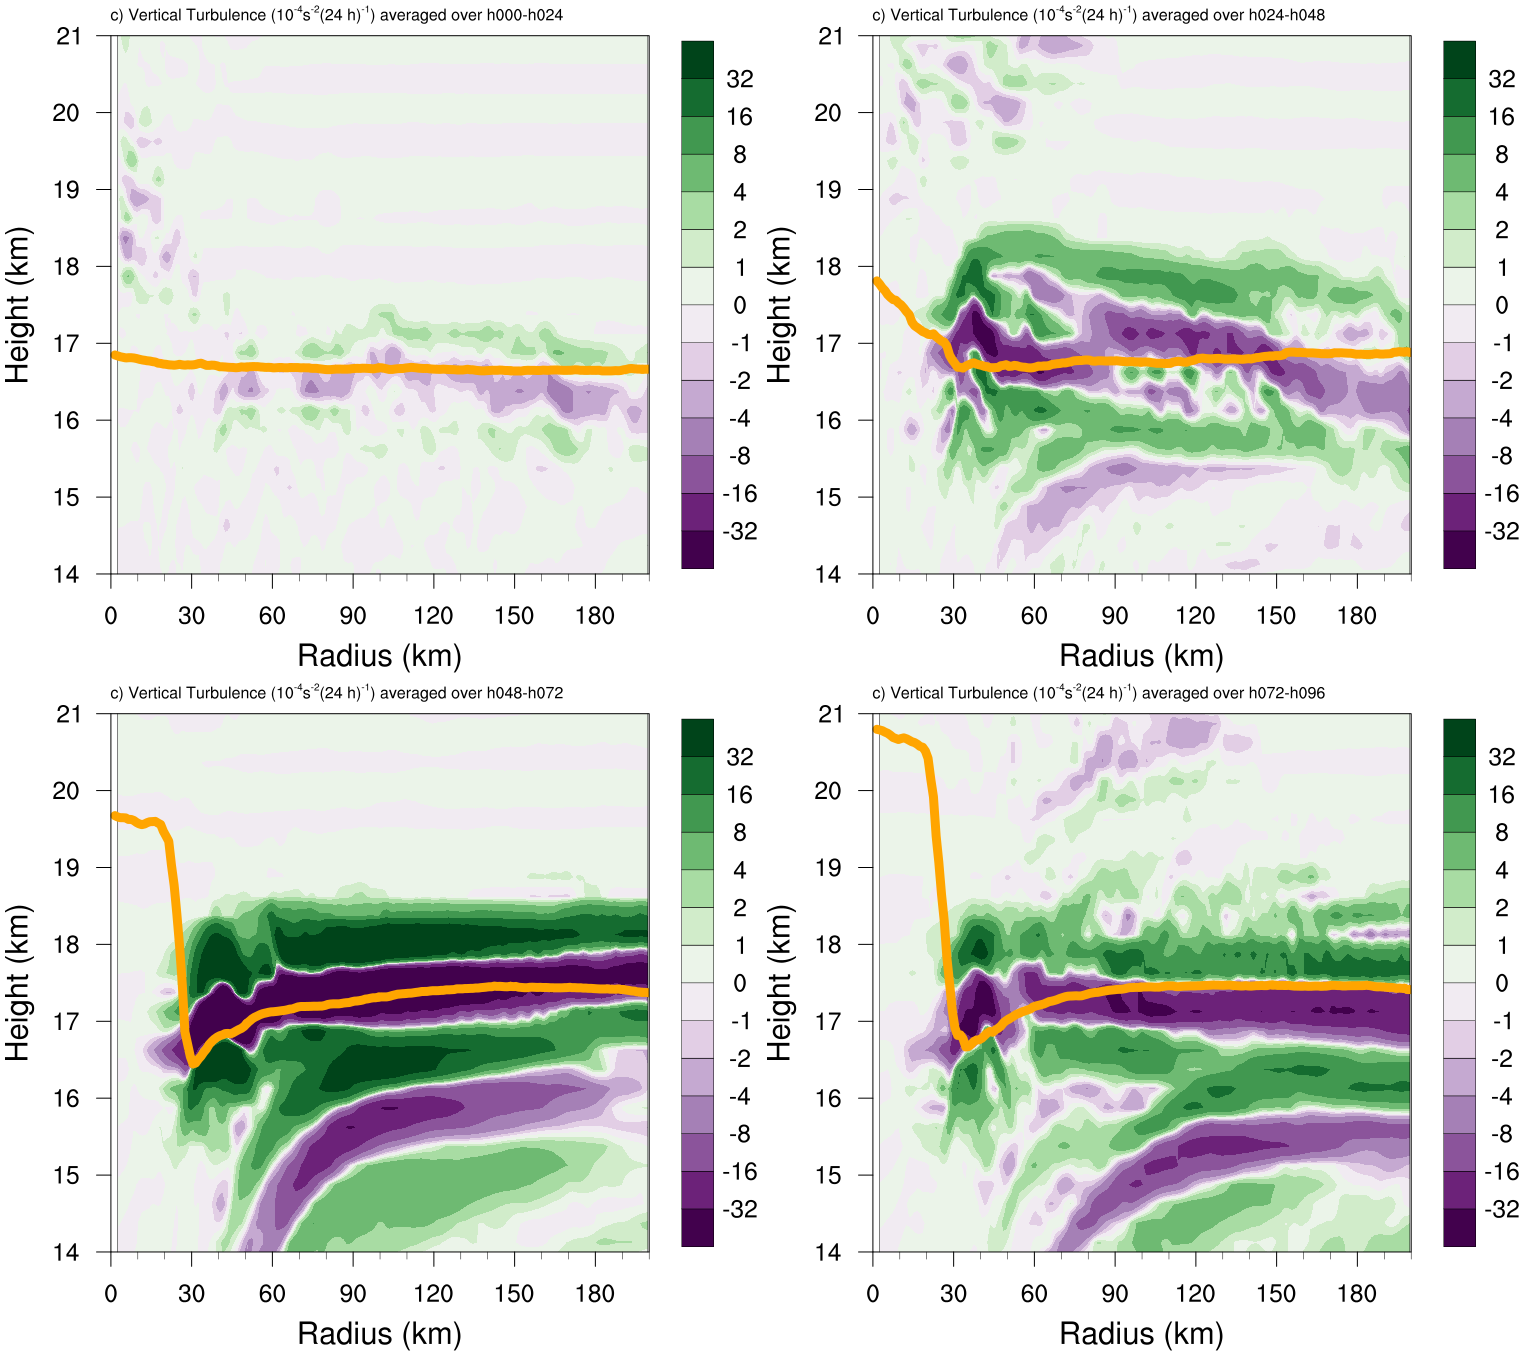
\includegraphics[width=39pc]{figures/turb-50m.png}}
%\appendcaption{A2}{The contribution of vertical turbulence to the $N^2$ variability (10\textsuperscript{-4} s\textsuperscript{-2} (24 h)\textsuperscript{-1}) averaged over (a) 0-24 hours, (b) 24-48 hours, (c) 48-72 hours, and (d) 72-96 hours for the simulation described in Appendix Ab. Orange lines represent the cold-point tropopause height averaged over the same time periods.}
%\label{fig:turb-50m}
%\end{figure*}

%\begin{figure}[t]
%\begin{figure}[t]
%\begin{figure}[t]
%  \noindent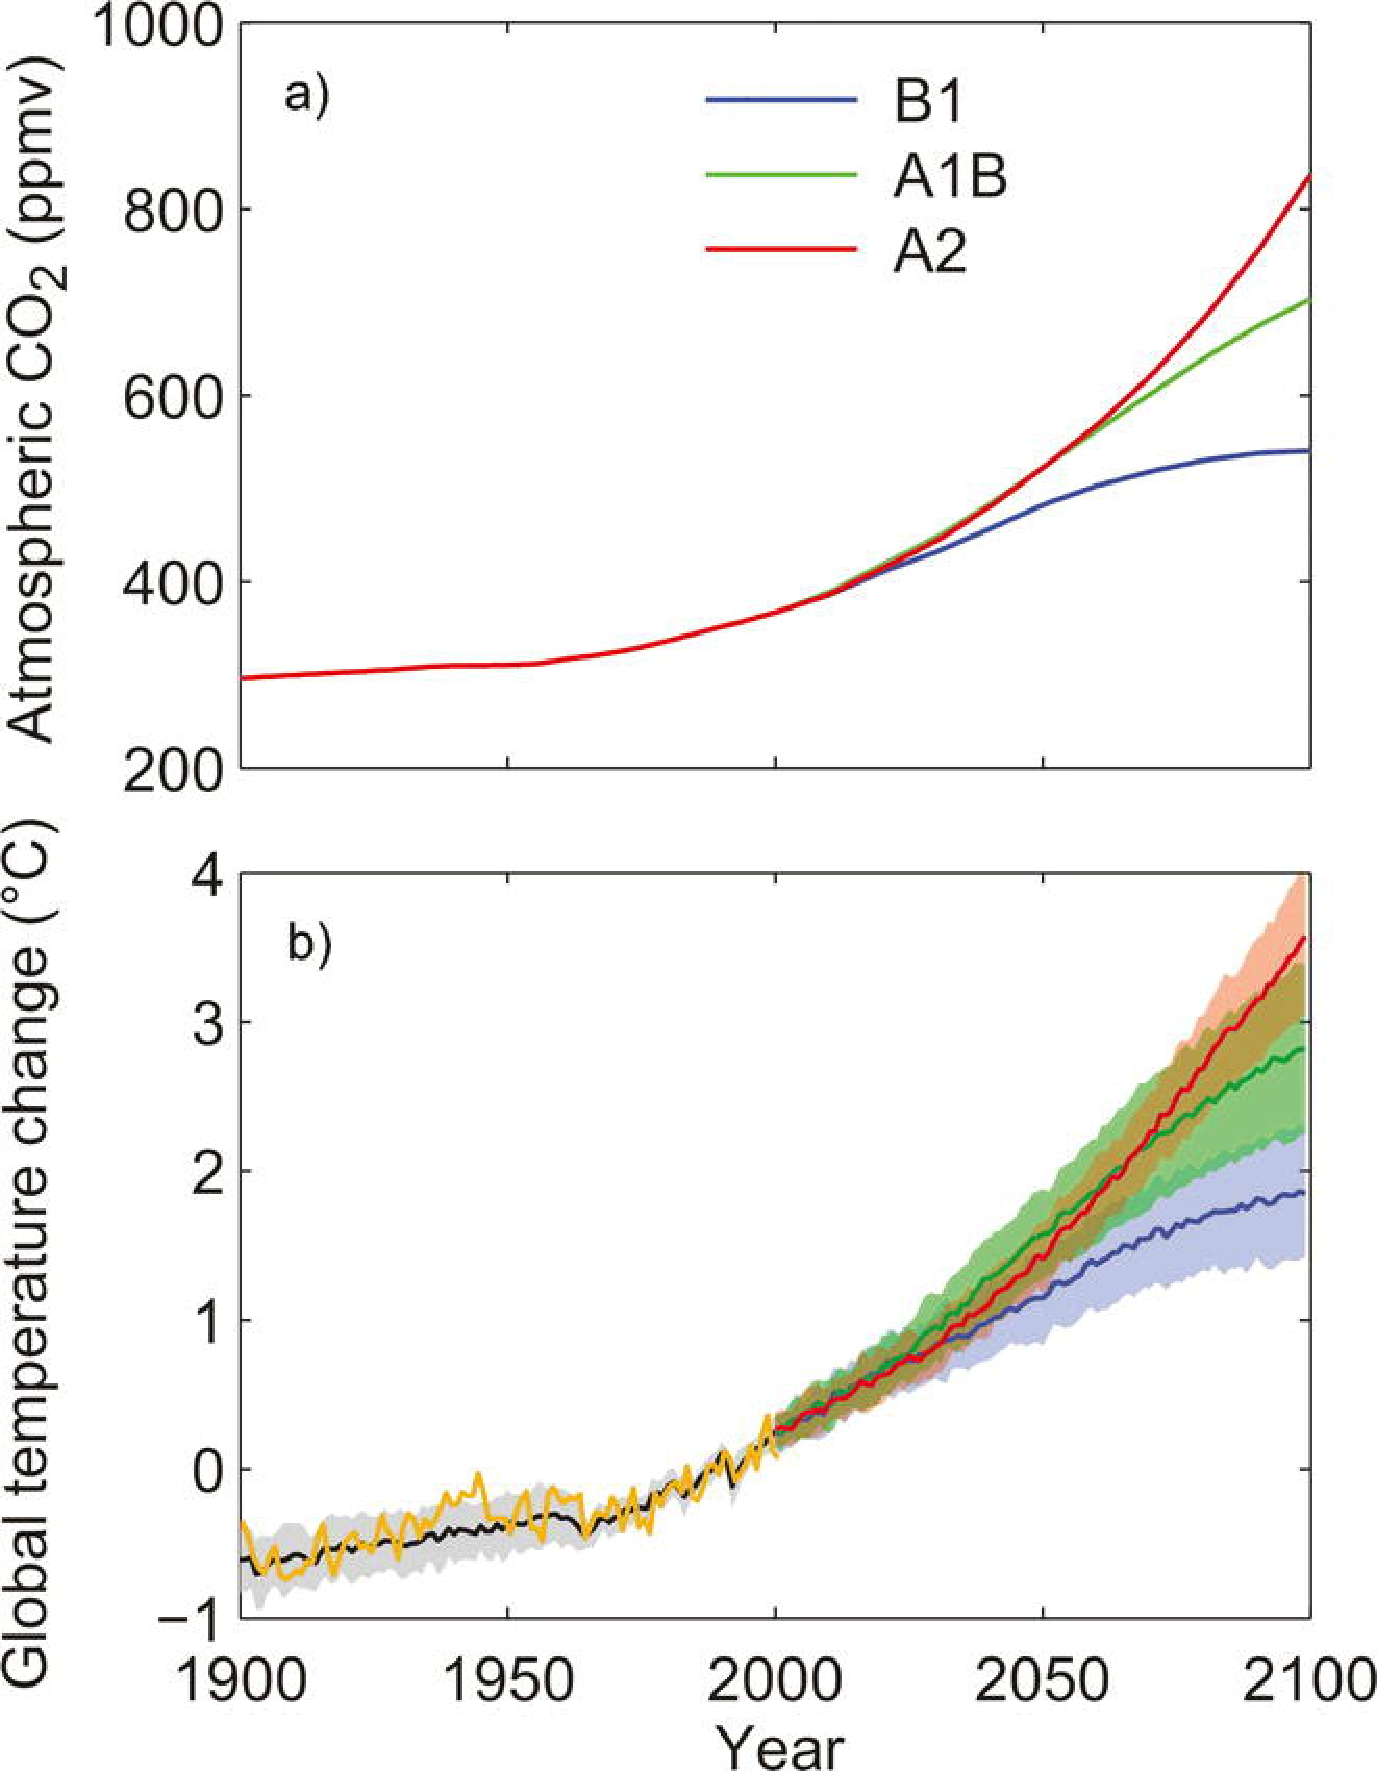
\includegraphics[width=19pc,angle=0]{figure01.pdf}\\
%  \caption{Enter the caption for your figure here.  Repeat as
%  necessary for each of your figures. Figure from \protect\cite{Knutti2008}.}\label{f1}
%\end{figure}

\end{document}
